% =============================================================================
%  MEMOIRE DE MASTER -- main file
%  Comparative Evaluation of Quantised Small Language Models for
%  Grammar-Constrained Command Parsing on Edge Hardware
%
%  COMPILE FROM thesis/ :
%     xelatex main_master  ->  biber main_master  ->  makeglossaries main_master
%     ->  xelatex main_master  ->  xelatex main_master
%
%  XeLaTeX (or LuaLaTeX) is REQUIRED -- polyglossia + an Arabic font render the
%  Arabic abstract. pdflatex will NOT build this.
%
%  Chapter structure is prd.md 3.1 verbatim (six chapters). Chapters not yet
%  written are listed commented-out below with their prd.md titles, so the
%  outline stays visible and the document still compiles.
% =============================================================================
\documentclass[openany,12pt,oneside]{extreport}

% =============================================================================
%  SHARED PREAMBLE -- \input by BOTH main_master.tex and main_ingenieur.tex.
%  There is deliberately ONE of these. The ESI templates in thesis/thesis_ex/
%  carry two forked copies of the same 120-line preamble, which is how they
%  drifted apart; do not reintroduce that by copying this file per document.
%
%  \documentclass does NOT belong here -- it must be the first line of each main.
% =============================================================================

% -- Engine note --------------------------------------------------------------
%  XeLaTeX or LuaLaTeX is REQUIRED (polyglossia + an Arabic font for the AR
%  abstract). pdfLaTeX will not build this document.
%  inputenc is deliberately absent: it is a pdfLaTeX package and conflicts with
%  XeLaTeX's native UTF-8. The ESI templates load it; that is a bug, not a model.

\usepackage{extsizes}
\usepackage{indentfirst}
\usepackage{csquotes}

% -- Maths and symbols --------------------------------------------------------
\usepackage{lmodern}
\usepackage{amsmath}
\usepackage{amsfonts}
\usepackage{amssymb}

% -- Floats, figures, tables --------------------------------------------------
\usepackage{graphicx}
\usepackage{float}
\usepackage{wrapfig}
\usepackage{caption}
\usepackage{subcaption}   % NOT subfigure: that package is obsolete and clashes
                          % with caption. The ESI templates still load subfigure.
\usepackage{tabularx}
\usepackage{array}
\usepackage{booktabs}
\usepackage{multirow}
\usepackage{longtable}
\usepackage{xltabular}    % longtable that still supports tabularx X columns:
                          % needed for any table taller than one page.
\usepackage{lscape}
\usepackage{pdflscape}
\usepackage{romannum}
\usepackage[normalem]{ulem}
\usepackage[bottom]{footmisc}

% -- Geometry -----------------------------------------------------------------
\usepackage[top=1.5cm, bottom=1.5cm, left=2.5cm, right=2.5cm, headheight=15pt]{geometry}

% -- Where figures are looked up ----------------------------------------------
\graphicspath{{shared/figures/}{master/figures/}{ingenieur/figures/}}

% -- Colour -------------------------------------------------------------------
\usepackage[table]{xcolor}
\definecolor{primarycolor}{RGB}{0,84,166}
\definecolor{accentcolor}{RGB}{220,100,0}
\definecolor{commentcolor}{RGB}{60,130,60}

% -- TikZ / plots -------------------------------------------------------------
%  tikz is loaded BEFORE any \usetikzlibrary / \tikzset. The PFE template in
%  thesis_ex/ comments out \usepackage{tikz} but still calls \usetikzlibrary
%  below it, which is why it does not compile.
\usepackage{tikz}
\usetikzlibrary{matrix,chains,positioning,decorations.pathreplacing,arrows,
                arrows.meta,fit,backgrounds,calc}
\tikzset{>=latex}
\usepackage{pgfplots}
\pgfplotsset{compat=1.18}

% -- Code listings ------------------------------------------------------------
\usepackage{listings}
\lstset{
    basicstyle=\ttfamily\footnotesize,
    backgroundcolor=\color{gray!10},
    commentstyle=\color{commentcolor},
    keywordstyle=\color{primarycolor}\bfseries,
    stringstyle=\color{accentcolor},
    numbers=left, numberstyle=\tiny\color{gray},
    stepnumber=1, numbersep=8pt,
    showstringspaces=false, breaklines=true,
    frame=single, rulecolor=\color{gray!30},
    captionpos=b, xleftmargin=15pt, xrightmargin=5pt
}

% -- Hyperlinks ---------------------------------------------------------------
\usepackage{hyperref}
\hypersetup{
  colorlinks = true, urlcolor = blue, linkcolor = blue, citecolor = blue
}

% -- Acronyms -----------------------------------------------------------------
\usepackage[acronym, automake, nonumberlist]{glossaries}

%  A two-column acronym table (Acronym | Definition) instead of the default
%  description list. Requires longtable, loaded above. The mains ask for this
%  by name: \printglossary[... style=acrolong].
\newglossarystyle{acrolong}{%
    \setglossarystyle{long}%
    \renewenvironment{theglossary}{%
        \begin{longtable}{p{3.5cm} p{11.5cm}}%
    }{%
        \end{longtable}%
    }%
    \renewcommand*{\glossaryheader}{%
        \toprule \bfseries Acronym & \bfseries Definition \\
        \midrule\endhead \bottomrule\endfoot
    }%
    \renewcommand{\glossentry}[2]{%
        \glsentryitem{##1}\glstarget{##1}{\glossentryname{##1}} &
        \glossentrydesc{##1} \\
    }%
}
\makeglossaries
%  Acronym DEFINITIONS are \input after \begin{document}, not here. The ESI
%  templates \include them in the preamble; \include issues \clearpage, which
%  is not legal before \begin{document}.

% -- Section depth ------------------------------------------------------------
%  \makeatletter is required: these names contain @, and this is a .tex file
%  \input in the preamble, where @ is not a letter. The ESI templates omit it.
\usepackage{titlesec}
\makeatletter
\def\toclevel@subsubsubsection{4}
\def\l@subsubsubsection{\@dottedtocline{4}{7em}{4em}}
\makeatother
%  secnumdepth 3, NOT 4. The chapters use \paragraph{...} as an unnumbered
%  lead-in ("Checkpoint selection."), which is the standard idiom. At depth 4
%  those get numbered, and because the chapters have no subsections in between
%  the numbers come out as "3.3.0.0.3 Checkpoint selection." The ESI templates
%  set 4; that is what produces those. tocdepth follows so the contents list
%  stops at subsubsection instead of listing every lead-in paragraph.
\setcounter{secnumdepth}{3}
\setcounter{tocdepth}{3}

% -- Chapter style ------------------------------------------------------------
%  Options: Sonny, Lenny, Glenn, Conny, Rejne, Bjarne, Bjornstrup
\usepackage[Glenn]{fncychap}

% -- Languages (LOADED LATE ON PURPOSE) --------------------------------------
%  polyglossia pulls in `bidi` as soon as an RTL language is declared, and bidi
%  REQUIRES that it be loaded after amsmath, amstext, caption, xcolor, colortbl
%  and friends. Declaring Arabic near the top of the preamble -- which is where
%  the ESI templates put it -- makes a cold build emit 17 "you have loaded
%  package X after bidi" errors. Keep this block below every package above.
%  babel is deliberately NOT loaded: polyglossia replaces it, and loading both
%  errors under XeLaTeX/LuaLaTeX. The ESI templates load both.
\usepackage{polyglossia}
\setdefaultlanguage{english}
\setotherlanguage[numerals=maghrib]{arabic}   % Latin digits inside Arabic text

%  Pick whichever Arabic font this machine actually has, rather than failing the
%  whole build on a missing font. If neither is installed the document still
%  compiles and the Arabic abstract renders in the default face (visibly wrong,
%  which is the point -- it tells you to install one).
\IfFontExistsTF{Amiri}{%
  \newfontfamily\arabicfont[Script=Arabic]{Amiri}%
}{%
  \IfFontExistsTF{Noto Sans Arabic}{%
    \newfontfamily\arabicfont[Script=Arabic]{Noto Sans Arabic}%
  }{%
    \GenericWarning{}{THESIS: no Arabic font found (tried Amiri, Noto Sans
      Arabic). The Arabic abstract will NOT render correctly. Install one
      before the final build: `sudo apt install fonts-hosny-amiri` or
      `fonts-noto-core`.}%
    %  Keep \arabicfont defined so the build still finishes: fall back to the
    %  roman family rather than naming a system font that may also be absent.
    \providecommand{\arabicfont}{\rmfamily}%
  }%
}


% -- Bibliography -------------------------------------------------------------
%  biblatex + biber over the ONE shared references.bib. sorting=none prints in
%  citation order; numeric-comp compresses [3,4,5] to [3-5]. Only entries a
%  given document actually cites are printed, which is why the two theses can
%  share one file without either listing references it never mentions.
\usepackage[backend=biber, sorting=none, style=numeric-comp]{biblatex}
\addbibresource{references.bib}

% =============================================================================
%  AUTHORING MARKERS -- all three are visible in the PDF and greppable in the
%  source. Nothing here should survive into the deposited document.
% =============================================================================

%  \TODO{...} -- a fact not yet available. Used by the chapters; see
%  .agents/skills/thesis-writing/SKILL.md on never hand-typing a number.
\newcommand{\TODO}[1]{{\bfseries\color{accentcolor}[TODO: #1]}}

%  \CHECK{...} -- a claim that needs verifying against a source or a result.
\newcommand{\CHECK}[1]{{\bfseries\color{accentcolor}[CHECK: #1]}}

%  \figtodo{...} -- a figure placeholder that compiles with no image file.
\newcommand{\figtodo}[1]{%
  \fbox{\parbox[c][3.6cm][c]{0.85\textwidth}{\centering\itshape\color{accentcolor}
  [FIGURE TO ADD]\\[4pt]\normalcolor\itshape #1}}}

% =============================================================================
%  NOTE ON \ifpfe
%  sample_thesis/ defines a \newif\ifpfe so one shared source file can word a
%  passage differently in each document. It is deliberately NOT defined here:
%  prd.md 3.2 states that no paragraph appears in both documents, so there are
%  no shared prose files for it to act on. Adding the toggle would invite
%  exactly the shared-paragraph writing that Table 3 forbids.
% =============================================================================


\title{Comparative Evaluation of Quantised Small Language Models for
       Grammar-Constrained Command Parsing on Edge Hardware}
\author{Tayeb Kahia}

\begin{document}

% Discourage overfull lines in a draft; revisit before the final build.
\tolerance=1
\emergencystretch=\maxdimen
\hyphenpenalty=10000
\hbadness=10000

% -- Title page ---------------------------------------------------------------
% =============================================================================
%  MASTER title page.
%  Facts below come from prd.md (student, supervisor, specialty, working title,
%  academic year). The JURY is not recorded anywhere in the repo -- the four
%  \CHECK markers below are deliberate and WILL render in the PDF. Replace them
%  before the depot; do not delete the markers without filling in the names.
% =============================================================================
\begin{titlepage}
% =============================================================================
%  ESI SBA cover-page header -- identical in both documents, so it lives once.
%  Wording and ordering are the school's; taken from the ESI templates in
%  thesis/thesis_ex/. Do not reword. The diploma, specialty, theme and jury
%  differ per document and live in each master/ or ingenieur/ titlepage.tex.
% =============================================================================
\centering
\begin{Arabic}
    {\normalsize \textsc{الجمهورية الشعبية الديمقراطية الجزائرية}}\\
\end{Arabic}
{\normalsize \textbf{République Algérienne Démocratique et Populaire}}\\

\begin{Arabic}
    {\normalsize \textsc{وزارة التعليم العالي و البحث العلمي}}\\
\end{Arabic}
{\normalsize \textbf{Ministère de l'Enseignement Supérieur et de la Recherche Scientifique}}\\

\begin{Arabic}
    {\large \textbf{المدرسة العليا للإعلام الآلي 08 ماي 1945 بسيدي بلعباس}}\\
\end{Arabic}
{\large \textbf{École Supérieure en Informatique \\-08 Mai 1945- Sidi Bel Abbès}\\}

\begin{figure}[ht]
\centering

\includegraphics[width=2.5cm]{Logo_ESI_SBA.png}
\end{figure}


\vspace{0.5cm}
{\Large \textbf{MASTER THESIS}}\\

\vspace{0.4cm}
{\large To obtain the diploma of \textbf{Master}\\}
{\large Field: \textbf{Computer Science}\\}
{\large Specialty: \textbf{Intelligence Artificielle et Sciences de Données (IASD)}\\}

\vspace{0.4cm}
{\Large \textbf{Theme}}\\
\rule{15cm}{0.2mm}\\
\vspace{0.4cm}
{\textbf{\large Comparative Evaluation of Quantised Small Language Models for
Grammar-Constrained Command Parsing on Edge Hardware}}\\
\rule{15cm}{0.2mm}\\
\vspace{0.2cm}

{\large Presented by:}\\
\vspace{0.2cm}
{\large \textbf{Tayeb KAHIA}}

\vspace{0.4cm}
{\large Submission Date: \textbf{September 2026}\\
In front of the jury composed of:}
\vspace{0.2cm}
\begin{center}
    {\large \textbf{\CHECK{jury president}} \hfill President\\}
    {\large \textbf{Prof. Belkacem KHALDI} \hfill Supervisor\\}
    {\large \textbf{\CHECK{co-supervisor, or delete this line}} \hfill Co-Supervisor\\}
    {\large \textbf{\CHECK{examiner}} \hfill Examiner\\}
\end{center}

\vspace{0.5cm}
{\normalsize \textit{Academic Year: 2025/2026}}
\end{titlepage}


% -- Front matter -------------------------------------------------------------
%  Numbering follows the ESI templates and sample_thesis: arabic throughout,
%  no roman front matter. Front matter is kept out of the TOC by dropping
%  tocdepth to -1 around it.
\pagenumbering{arabic}
\addtocontents{toc}{\protect\setcounter{tocdepth}{-1}}

% Dedication -- shared by both documents.
\thispagestyle{empty}
\vspace*{5cm}
\begin{flushright}
\itshape
To my mother,\\
whose love, patience and du'a\\
have carried me through every step of this path.\\[0.4cm]
This work is yours as much as it is mine.
\end{flushright}
\newpage

% Acknowledgements -- shared by both documents.
\thispagestyle{empty}
\vspace*{2cm}
\begin{center}{\Huge\bfseries Acknowledgements}\end{center}
\vskip 1cm
\noindent First and foremost, all praise and thanks are due to Allah (\emph{Alhamdulillah}), who
granted me the health, the patience and the strength to carry this work through to its end.

\vspace{0.3cm}
\noindent I express my deepest gratitude to my supervisor, Prof.~Belkacem KHALDI. His help went
far beyond what a page of acknowledgements can record. He was generous with his time, patient with
my questions, and constant in his encouragement at every stage of this work. His guidance gave the
work its direction, and his trust gave me the confidence to see it through. For all of this, I am
sincerely and lastingly grateful.

\vspace{0.3cm}
\noindent I thank the members of the jury for the time they have given to reading and evaluating
this work, and the \'Ecole Sup\'erieure en Informatique -- 08 Mai 1945 -- Sidi Bel Abb\`es and its
teaching staff for the training on which it rests.

\vspace{0.3cm}
\noindent To my mother, above all. Her unwavering support, her patience and her constant du'a
carried me through every stage of this work, and whatever I have achieved I owe first to her. To my
sister, thank you for your encouragement and your presence throughout.

\vspace{0.3cm}
\noindent To my friends Yacine and Zineddine, thank you for your support. And to all my
fifth-year classmates, especially Salah and Mohammed: thank you for the years we shared and for
standing by me.

\newpage

% English abstract -- Mémoire de Master.
% One paragraph of context, one of what was done, one of what was found.
% Numbers here must trace to results/*.csv; see the thesis-writing skill.
\thispagestyle{empty}
\vspace*{4cm}
\begin{center}{\Huge\bfseries Abstract}\end{center}
\vskip 1cm
\noindent A drone swarm commanded by voice needs a parser that turns a transcribed utterance into an
executable command on the vehicle's own hardware, where every added parameter costs latency and a
wrong output is a control error. This thesis asks what the accuracy--efficiency trade-off is across
small language models of 0.36--1.2~B parameters, fine-tuned for drone-swarm command parsing and
quantised for CPU-only execution on a Raspberry~Pi~5.

\vspace{0.3cm}
\noindent A frozen command schema is paired with a matched grammar that constrains decoding, so
that structural validity is a property of the decoder. A label-first dataset pipeline produces the
training and test data, with splits assigned by template family and a golden test set of 200
recorded commands. Four models are fine-tuned under one recipe; three are quantised at two levels
and measured on the board, and the fourth, matched in size to one of them, separates model family
from size. A selection rule fixed before any result existed chooses the configuration to deploy.

\vspace{0.3cm}
\noindent The trade-off reduces to two non-dominated configurations, SmolLM2-360M and
Qwen2.5-0.5B, and the rule deploys Qwen2.5-0.5B at Q4\_K\_M, at 0.935 exact match on the golden
set. SmolLM2-360M is faster and 17.5 percentage points less accurate, a significant difference;
Llama-3.2-1B is slower, and its lower accuracy on the golden set is not statistically established.
The selection is made on accuracy against re-baselined constraints: the selected configuration
misses the 2{,}500~ms end-to-end latency budget by 622~ms, and the budget is re-baselined to the
measured 3{,}122~ms. Every configuration misses the safe-failure and false-command requirements,
emitting a well-formed command rather than declining; a confidence gate on the decoder's output is
the first step proposed.

\vspace{1cm}
\providecommand{\keywords}[1]{\textbf{\textit{Keywords---}} #1}
\keywords{small language models; edge inference; quantisation; grammar-constrained decoding;
command parsing; Raspberry Pi 5; drone swarm; Pareto frontier.}
\newpage

% French abstract (résumé) -- Mémoire de Master. Same content as abstract.tex, in French.
\thispagestyle{empty}
\vspace*{4cm}
\begin{center}{\Huge\bfseries Résumé}\end{center}
\vskip 1cm
\noindent Un essaim de drones commandé à la voix a besoin d'un analyseur qui transforme un énoncé
transcrit en une commande exécutable sur le matériel embarqué du véhicule, où chaque paramètre
supplémentaire coûte de la latence et où une sortie erronée est une erreur de pilotage. Ce mémoire
étudie le compromis entre précision et efficacité parmi de petits modèles de langage de 0,36 à
1,2~milliard de paramètres, affinés pour l'analyse de commandes d'essaims de drones et quantifiés
pour une exécution sur le seul processeur central d'un Raspberry~Pi~5.

\vspace{0.3cm}
\noindent Un schéma de commandes figé est associé à une grammaire qui lui correspond et contraint le
décodage, de sorte que la validité structurelle est une propriété du décodeur. Une chaîne de
constitution des données qui part des étiquettes produit les données d'entraînement et de test,
avec des partitions attribuées par famille de gabarits et un jeu de test de référence de
200~commandes enregistrées. Quatre modèles sont affinés selon une même recette~; trois sont
quantifiés à deux niveaux, leurs artefacts Q4\_K\_M sont chronométrés sur la carte, et le
quatrième, de taille appariée à l'un d'eux, mesure une différence entre familles de modèles à
taille fixée. Une règle de sélection fixée
avant l'obtention de tout résultat désigne la configuration à déployer.

\vspace{0.3cm}
\noindent Parmi les trois modèles chronométrés sur la carte, le compromis en Q4\_K\_M se réduit à
deux configurations non dominées, SmolLM2-360M et Qwen2.5-0.5B, et la règle déploie Qwen2.5-0.5B en
Q4\_K\_M, avec une correspondance exacte de 0,935 sur le jeu de référence, évaluée sur le texte de
référence des commandes. SmolLM2-360M est plus rapide et moins précis de 17,5~points de pourcentage, une
différence significative~; Llama-3.2-1B est plus lent, et sa précision inférieure sur le jeu de
référence n'est pas statistiquement établie. La sélection se fait sur la précision, face à des
contraintes redéfinies d'après les mesures~: la configuration retenue dépasse de 622~ms le budget
de latence de bout en bout de 2\,500~ms, et ce budget est redéfini à la valeur mesurée de
3\,122~ms. Aucune configuration ne satisfait les exigences de taux d'échec sûr et de taux de fausses
commandes, et ces deux écarts relèvent d'une même tendance~: lorsqu'une configuration se trompe ou
que l'entrée est hors domaine, elle émet une commande bien formée au lieu de s'abstenir. Un seuil de
confiance appliqué à la sortie du décodeur est la première étape proposée.

\vspace{1cm}
\providecommand{\motscles}[1]{\textbf{\textit{Mots-clés---}} #1}
\motscles{petits modèles de langage~; inférence embarquée~; quantification~; décodage contraint
par grammaire~; analyse de commandes~; Raspberry Pi~5~; essaim de drones~; front de Pareto.}
\newpage

% Arabic abstract -- Mémoire de Master.
% Requires XeLaTeX/LuaLaTeX and an Arabic font; see shared/preamble.tex.
\thispagestyle{empty}
\vspace*{4cm}
\begin{center}{\Huge\bfseries \begin{Arabic}ملخص\end{Arabic}}\end{center}
\vskip 1cm
\begin{Arabic}
يحتاج سرب من الطائرات المسيّرة يُقاد بالصوت إلى محلِّل يحوّل العبارة المنطوقة بعد تفريغها نصيًا
إلى أمر قابل للتنفيذ على العتاد المدمج في المركبة نفسها، حيث تكلّف كل معلمة إضافية زمنًا في
الاستجابة، ويكون كل خرج خاطئ خطأً في التحكم. تتناول هذه المذكرة المفاضلة بين الدقة والكفاءة لدى
نماذج لغوية صغيرة تتراوح بين \textenglish{0.36} و\textenglish{1.2} مليار معلمة، مضبوطة ضبطًا
دقيقًا لتحليل أوامر أسراب الطائرات المسيّرة، ومُكمَّمة للتنفيذ على المعالج المركزي وحده لحاسوب
\textenglish{\mbox{Raspberry Pi 5}}.

\vspace{0.3cm}
يُقرَن مخطط أوامر مُثبَّت بقواعد نحوية مطابقة له تقيّد عملية فك الترميز، بحيث تصبح الصحة البنيوية
خاصيةً لمفكّك الترميز. وتُنتج سلسلةٌ لبناء البيانات تنطلق من التسميات بياناتِ التدريب والاختبار، مع
تقسيمات تُسنَد حسب عائلة القوالب، ومجموعة اختبار مرجعية من \textenglish{200} أمر مسجَّل. تُضبط أربعة
نماذج ضبطًا دقيقًا وفق وصفة واحدة؛ ويُكمَّم ثلاثة منها بمستويين وتُقاس على الجهاز، أما الرابع،
المماثل في الحجم لأحدها، فيفصل أثر عائلة النموذج عن أثر الحجم. وتختار قاعدةُ انتقاءٍ ثُبِّتت قبل
وجود أي نتيجة التهيئةَ التي تُنشر.

\vspace{0.3cm}
تنحصر المفاضلة في تهيئتين غير مُهيمَن عليهما، هما \textenglish{\mbox{SmolLM2-360M}}
و\textenglish{\mbox{Qwen2.5-0.5B}}، وتنشر القاعدة \textenglish{\mbox{Qwen2.5-0.5B}} بتكميم
\textenglish{Q4\_K\_M}، بمطابقة تامة قدرها \textenglish{0.935} على المجموعة المرجعية. والنموذج
\textenglish{\mbox{SmolLM2-360M}} أسرع وأقل دقة بـ\textenglish{17.5} نقطة مئوية، وهو فرق دالّ إحصائيًا؛ أما
\textenglish{\mbox{Llama-3.2-1B}} فأبطأ، ودقته الأدنى على المجموعة المرجعية غير مُثبتة إحصائيًا. ويتم
الانتقاء على أساس الدقة، مقابل قيود أُعيد ضبطها على القيم المقيسة: إذ تتجاوز التهيئة المختارة ميزانية
زمن الاستجابة من طرف إلى طرف البالغة \textenglish{2{,}500} ميلي ثانية بمقدار \textenglish{622} ميلي
ثانية، ويُعاد ضبط هذه الميزانية على القيمة المقيسة البالغة \textenglish{3{,}122} ميلي ثانية. ولا
تستوفي أي تهيئة متطلبات معدل الإخفاق الآمن ومعدل الأوامر الزائفة، إذ تُصدر أمرًا سليم البنية بدل
الامتناع عن الإجابة؛ وتُعدّ بوابة ثقة تُطبَّق على خرج مفكّك الترميز أولى الخطوات المقترحة.

\vspace{1cm}
\noindent\textbf{الكلمات المفتاحية:} النماذج اللغوية الصغيرة؛ الاستدلال على الأجهزة الطرفية؛ التكميم؛
فك الترميز المقيَّد بالقواعد النحوية؛ تحليل الأوامر؛ \textenglish{\mbox{Raspberry Pi 5}}؛ سرب الطائرات
المسيّرة؛ جبهة باريتو.
\end{Arabic}
\newpage


% -- Contents -----------------------------------------------------------------
% Back to the preamble's tocdepth (3). Restoring 4 here would override it and
% list every \paragraph lead-in -- "Synthesis.", "Gap." -- in the contents.
\addtocontents{toc}{\protect\setcounter{tocdepth}{3}}
\tableofcontents
\listoffigures
\listoftables

% -- Acronyms -----------------------------------------------------------------
% =============================================================================
%  ACRONYM DEFINITIONS -- shared by both theses.
%  \input AFTER \begin{document} (see shared/preamble.tex for why \include in
%  the preamble is wrong). \makeglossaries is already called in the preamble.
%
%  Use \gls{key} for "SLM" after first use, \acrfull{key} for the long form.
%  Every acronym below is one that actually appears in a written chapter --
%  do not pad this list with terms the documents never use.
% =============================================================================

% -- Models and inference -----------------------------------------------------
\newacronym{slm}{SLM}{Small Language Model}
\newacronym{llm}{LLM}{Large Language Model}
\newacronym{lora}{LoRA}{Low-Rank Adaptation}
\newacronym{ggml}{GGML}{Georgi Gerganov Machine Learning (tensor library)}
\newacronym{gguf}{GGUF}{GGML Universal File (quantised weight format)}
\newacronym{bnf}{BNF}{Backus--Naur Form}
\newacronym{gbnf}{GBNF}{GGML Backus--Naur Form (grammar format)}

% -- Speech and audio ---------------------------------------------------------
\newacronym{stt}{STT}{Speech To Text}
\newacronym{tts}{TTS}{Text To Speech}
\newacronym{vad}{VAD}{Voice Activity Detection}
\newacronym{wer}{WER}{Word Error Rate}
\newacronym{snr}{SNR}{Signal-to-Noise Ratio}
\newacronym{rms}{RMS}{Root Mean Square}

% -- Hardware -----------------------------------------------------------------
\newacronym{sbc}{SBC}{Single-Board Computer}
\newacronym{cpu}{CPU}{Central Processing Unit}
\newacronym{gpu}{GPU}{Graphics Processing Unit}
\newacronym{uav}{UAV}{Unmanned Aerial Vehicle}
\newacronym{pid}{PID}{Proportional-Integral-Derivative (controller)}

% -- Requirements and evaluation ----------------------------------------------
\newacronym{fr}{FR}{Functional Requirement}
\newacronym{nfr}{NFR}{Non-Functional Requirement}
\newacronym{em}{EM}{Exact Match}
\newacronym{crr}{CRR}{Command Recognition Rate}
\newacronym{fa}{FA}{False Acceptance}
\newacronym{roc}{ROC}{Receiver Operating Characteristic}

% -- Formats ------------------------------------------------------------------
\newacronym{json}{JSON}{JavaScript Object Notation}
\newacronym{sha}{SHA}{Secure Hash Algorithm}

\printglossary[type=\acronymtype, title=List of Acronyms, style=acrolong]
\clearpage

% -- Chapters (prd.md 3.1) ----------------------------------------------------
% Introduction
% Scaffold only --- section structure from prd.md 3.1, ownership from Table 3.
% The NOTE comments say what belongs in each section and where the material already is.
% Delete each NOTE as you fill the section. Prose is yours to write.

\chapter{Introduction}

\section{The edge-inference problem}
% NOTE: Why run a language model on a Raspberry Pi 5 at all: no network, no cloud latency, no data
%       leaving the aircraft. Source: prd.md 1.
% NOTE: Ground the difficulty with a measured number, not an assertion: spikes/reports/S1 has
%       Qwen2.5-0.5B Q4_K_M at 20.97 tok/s on 3 threads against a >=20 tok/s budget -- a 4.9%
%       margin. That thin margin IS the problem statement.

\section{Why structured output matters for robot control}
% NOTE: A chat model that is 95% right about JSON is 100% useless to a flight controller. Motivate
%       the schema-as-contract idea that C1 formalises.
% NOTE: spikes/reports/S3 is the evidence: base models degenerating into unbounded id lists. Cite it
%       as motivation, not as a result.

\section{Objectives}
% NOTE: RQ1 verbatim from prd.md:113. This document owns RQ1 only (Table 2); RQ2/RQ3 belong to the
%       Ingenieur.

\section{Contributions}
% NOTE: C1, C2, C3 from prd.md:121-123. C4 is the Ingenieur's -- do not claim it here.
% NOTE: State each as what was DONE, not what was intended.

\section{Structure of this document}
% NOTE: One short paragraph, five chapters.


\chapter{Related work}
\label{chap:related-work}

This chapter reviews the four bodies of work this thesis draws on: benchmarks of language-model
inference on \glspl{sbc}, post-training quantisation, grammar-constrained decoding, and
spoken-language understanding. Each section states what its literature establishes and what it
leaves unmeasured for this task and this hardware. Section~\ref{sec:positioning} combines the four
into the gap that RQ1 addresses and maps each contribution onto it.

\section{Edge language-model inference and single-board-computer benchmarking}
Running a language model without a network connection or a data-centre accelerator is now an
active subject of measurement. A recent benchmark evaluates twenty-five quantised language
models on three \glspl{sbc} under two inference runtimes, Ollama and
Llamafile~\cite{sbc2025}. It finds that such boards reliably support models of up to roughly
1.5~billion parameters, with larger models dropping to a few tokens per second. On the
one board where both runtimes were compared, Llamafile reached up to four times the throughput of
Ollama~\cite{sbc2025}. That result sets the shape of the problem this thesis inherits. On
\gls{cpu}-only edge hardware throughput is the scarce resource, and the models that fit within it
are small ones; the inference runtime is a lever on it of the same order as the choice of model.

What that benchmark does not report is what happens to a model once it is asked to do something
with the tokens it produces. Its outcome metrics describe speed and resource use, measured
independently of any downstream task. A configuration that clears a throughput floor and one that
clears it while producing ungrammatical or semantically wrong output are therefore
indistinguishable in its tables. This thesis narrows the scope to one task, one device, and four
fine-tuned models (Qwen2.5-0.5B~\cite{qwen25}, SmolLM2-360M~\cite{smollm2},
Llama-3.2-1B~\cite{llama32}, and H2O-Danube3-500M~\cite{danube3}). In exchange it measures what
the benchmark does not: \gls{em}, intent and slot F1, schema validity, and false-command rate.
Three of those models are carried through to quantised artefacts and timed against the
20~tok/s throughput floor of Chapter~\ref{chap:introduction}. The fourth, a parameter-matched
control, is reported at fp16 only, because llama.cpp segments its prompt differently from the
tokeniser it was trained under (Chapter~\ref{chap:method}). The accuracy cost of meeting a
throughput budget on an \gls{sbc} is thus treated as a quantity to be measured, not
assumed from a benchmark that reports throughput alone.

The runtime that makes this measurement possible on the target hardware is llama.cpp, a C/C\,++
inference engine for quantised language models that runs on a \gls{cpu} without external
dependencies, and in particular without a \gls{gpu} driver~\cite{llamacpp}. Its \gls{gguf}
weight format and its quantisation schemes shrink the weights a Raspberry~Pi~5 must read for every
decoded token; Section~\ref{sec:quantisation} takes up what those schemes cost in accuracy.

\section{Quantisation}
\label{sec:quantisation}
% NOTE: \cite{llamacpp} below is correct and load-bearing, not a placeholder. No
%       peer-reviewed analysis of the k-quant scheme itself appears to exist, so the
%       runtime is the primary source for the SCHEME DESCRIPTION. \cite{gptq} and
%       \cite{awq} carry the field-level claims around it. Do not 'fix' this.
Post-training quantisation is the established route to reducing a trained model's memory
footprint~\cite{gptq}, and on-device deployment is one of its stated motivations~\cite{awq}.
This thesis deploys two of llama.cpp's \gls{gguf} quantisation formats. Q8\_0, a legacy format,
stores weights in blocks of 32 at eight bits with one scale per block, 8.5~bits per weight in
all. Q4\_K\_M belongs to the K-quant family, which stores weights in super-blocks of 256 with
quantised per-sub-block scales, 4.5~bits per weight at the four-bit level~\cite{llamacpp}. Its
target is four bits for most tensors. A fixed rule raises the output projection, and a subset of
the attention-value and feed-forward down-projection tensors chosen by layer position, to six
bits~\cite{llamacpp}. A K-quant also requires each tensor's rows to divide into whole
super-blocks: a tensor whose row length is not a multiple of 256 falls back to a legacy format,
five bits in place of four and eight in place of six~\cite{llamacpp}. The name Q4\_K\_M therefore
denotes an allocation recipe rather than a bit width, and in a model whose hidden dimension is not
a multiple of 256 most of the weights end up at five or eight bits. The recipe allocates bits by
tensor role, position and shape, not by any measurement of error. The method literature measures
instead: it finds that protecting the roughly one percent of weight channels that activation
statistics mark as salient greatly reduces quantisation error~\cite{awq}.

The runtime's documentation states that the accuracy cost of its formats is usually measured as
a perplexity or a Kullback--Leibler divergence against the unquantised model~\cite{llamacpp},
not as a change in accuracy on a downstream task. A perplexity number averaged over held-out text
says how much less confident the quantised model is about the next token in general. It does not
say whether the intent assigned to a spoken command, or the slot values filled in, still match the
ground truth once the weights have been rounded to lower precision. This thesis needs the
second number, because its model's output is acted on by a swarm controller after automatic
validation, not read by a person. The papers introducing post-training quantisation methods report
their cost mainly in generic terms: SpQR reports a relative perplexity loss of under one
percent~\cite{spqr}, and GPTQ reports perplexity together with zero-shot accuracy on generic
benchmarks such as LAMBADA, ARC and PIQA~\cite{gptq}.

Evaluation studies have since measured downstream accuracy under quantisation at
scale~\cite{kurtic2025}, and for llama.cpp's own formats specifically~\cite{kurt2026}. Their
models are mostly of eight billion parameters and above, scored on general-purpose reasoning,
knowledge and coding suites with the decoder unconstrained; the smallest model either study
evaluates has 1.5~billion parameters~\cite{kurtic2025}. Small models have also been studied
directly: a benchmark of quantisation at sub-billion scale, which includes Qwen2.5-0.5B, finds that
small models differ from large ones in their sensitivity to quantisation, so that methods tuned on
large models transfer poorly~\cite{slmquant}. None of these studies scores a structured
command-parsing task by \gls{em}, intent and slot F1, or schema validity, and none decodes under
a grammar. Chapter~\ref{chap:results} measures the accuracy cost of the whole deployment pipeline
on that task, for the three quantised models at both levels, as part of Contribution~C3.
Section~\ref{sec:quantisation-procedure} explains why that pipeline cost is not the cost of
quantisation alone, and why it is not to be read against the studies above.

\section{Constrained decoding}
\label{sec:constrained-decoding}
Grammar-constrained generation restricts, at every decoding step, the set of tokens the model is
allowed to sample to those consistent with a formal grammar, so that no output can leave the
grammar's language regardless of what the model would otherwise have produced. The technique has
been applied to structured language-processing tasks without fine-tuning~\cite{geng2023}. Its
formulations compile a regular expression or a context-free grammar into an automaton over the
vocabulary and mask the decoder against it~\cite{willard2023,koo2024}, with correctness results
for the language classes such a construction covers~\cite{koo2024}. \Gls{gbnf} is the grammar
formalism llama.cpp implements it with: a context-free grammar applied at each decoding step to
mask the tokens it cannot accept. Its per-step cost depends on the grammar's
structure, and the documentation warns that some rule shapes make sampling slow~\cite{llamacpp}.
This is a different mechanism from prompting a model to produce well-formed output and then
checking the result: the grammar acts inside the sampling loop, before an invalid token can be
emitted, not after a full sequence has been generated.

That difference in mechanism is also a difference in the kind of claim that can be made about
structural validity. Without a grammar, whether a model's output parses against a schema is an
empirical question, answered by counting how often it does so on some test set, and the answer
can change whenever the input distribution changes. With a grammar compiled from the same schema,
the question is closed by construction: no string outside the grammar's language is reachable, on
any input, provided the generation cap exceeds the longest string that language contains. The
bounded grammar of Section~\ref{sec:schema} makes that length finite. Constrained decoding thus
moves structural validity from a rate that fine-tuning and a favourable test set can inflate to a
property the decoder enforces independently of both. The grammar ablation of
Chapter~\ref{chap:results} decodes the same fine-tuned models with and without the grammar, and so
measures how often they leave the format when nothing prevents them.

That property has a cost, which is why the ablation reports accuracy as well as validity.
Constraining the decoder alters the distribution the model samples from: outputs remain
grammatical, but their relative likelihoods no longer track what the unconstrained model would
have assigned, so a grammar can make a structurally valid command more likely without making the
correct one more likely~\cite{park2024}. Format restriction has separately been observed to
degrade accuracy on reasoning tasks, more so as the restriction tightens, while classification
tasks were in some cases helped by it~\cite{tam2024}. The size of either effect on a given task
does not follow from that literature. The distortion result establishes that the effect exists,
not how large it is, and the format-restriction study finds even its direction task-dependent.
Of the two task types it compares, classification is the closer to parsing a command into one of
ten intents. Chapter~\ref{chap:results} therefore reports accuracy with and without the grammar,
not structural validity alone.

\section{Spoken-language understanding for robotics}
\label{sec:slu-robotics}
Parsing an utterance into an intent and a set of slot values is an established formulation in
spoken-language understanding, not one this thesis introduces. A survey of the field treats the
extraction of this semantic frame as the object of the task, and classifies methods by whether they
model intent and slots separately or jointly~\cite{qin2021}. MASSIVE, a dataset of one million
utterances in 51 languages labelled with 60 intents and 55 slot types, is built around the same
formulation~\cite{massive}. Its baselines, encoders of 258 to 580~million parameters, reach
locale-averaged intent accuracies of 85.1--86.1\% and slot F1 of 73.6--76.8\%, but \gls{em}
of only 63.7--66.6\%~\cite{massive}. For the single-utterance commands considered here, a spoken
instruction to a robot has the same shape: one intent from a fixed set and a handful of slot
values. Language-model control of robots and aircraft more broadly is reviewed in the
\emph{M\'emoire d'Ing\'enieur}.

What differs in this deployment is the setting, not the shape of the task. MASSIVE's baselines are
trained on data-centre \glspl{gpu}, decoded without a grammar, and scored with no latency or
memory limit~\cite{massive}. Their lowest figure is \gls{em}, and it is the metric a controller
depends on, since a command with one wrong slot is a wrong command. Here the model has to
run offline, at sub-billion-parameter scale, within the throughput budget of a Raspberry~Pi~5, and
its output is acted on by the swarm controller after automatic validation, with no person reading
it first. No existing corpus covers this command vocabulary (Section~\ref{sec:dataset}). That the
task shape is well studied does not show that it can be solved at this size and within this
budget, with an error rate low enough for output that no person reads. The evaluation protocol of
Chapter~\ref{chap:method} is built to answer that question.

\section{Positioning}
\label{sec:positioning}

\paragraph{Synthesis.} Each of the four literatures reviewed in this chapter answers its own
question. Benchmarking on \glspl{sbc} has found that such boards reliably serve models of up to
about 1.5~billion parameters, and that on one board the choice of runtime changed throughput by up
to four times~\cite{sbc2025}. Post-training quantisation is the established way to shrink a trained
model~\cite{gptq}, with on-device deployment among its motivations~\cite{awq}. Its cost is reported as perplexity and generic zero-shot accuracy by
the papers introducing the methods~\cite{spqr,gptq}, and as accuracy on general-purpose suites by
the studies evaluating them, including at sub-billion scale~\cite{kurtic2025,kurt2026,slmquant}.
Grammar-constrained decoding makes a model's output structurally valid by construction rather than
by the accuracy of the model that produced it~\cite{willard2023,koo2024}, at costs its own
literature documents: a distorted sampling distribution~\cite{park2024} and, on reasoning tasks,
lower accuracy~\cite{tam2024}. Intent and slot parsing
is an established task formulation, with a large multilingual benchmark built for
it~\cite{massive}. Some pairs of these literatures have already been combined: quantisation with
\gls{cpu} inference and downstream accuracy~\cite{kurt2026}, quantisation with small
models~\cite{slmquant}, and format restriction with task accuracy~\cite{tam2024}. No study
reviewed here combines all four.

\paragraph{Gap.} The gap lies in that combination: a sub-billion model fine-tuned to a command
schema, quantised to a format an \gls{sbc} can serve, decoded under a grammar, and
scored on task metrics alongside its throughput on the board. The single-board-computer benchmark
reviewed here reports throughput without reference to any task, so it cannot say what a
configuration that meets a throughput floor costs in task accuracy. The quantisation studies report
accuracy on general-purpose benchmarks with the decoder unconstrained, not \gls{em}, intent and
slot F1, or schema validity on a command-parsing task. The constrained-decoding studies reviewed here
evaluate grammars and format restrictions on models that were not fine-tuned to the target format, so what a grammar still adds
once fine-tuning has taught a model that format is not reported. Intent-and-slot benchmarks such as
MASSIVE are scored on data-centre hardware without a latency budget or a grammar, and no existing
corpus covers this command vocabulary. Choosing a model to deploy on this hardware requires all
four quantities measured together, on the configuration that is actually deployed.

\paragraph{Delta.} The three contributions of this thesis address that gap as follows.
Contribution C1, the frozen command schema and its matched, bounded \gls{gbnf} grammar, makes
structural validity on this task a property of the decoder. The grammar ablation, run with the
harness of Contribution C3, decodes the same fine-tuned, quantised models with and without that
grammar, and so reports what the grammar adds once fine-tuning has taught the models the format.
Contribution C2, the label-first dataset (each label written before the sentences that express
it), supplies what a general-purpose corpus such as MASSIVE does not: training and test data for
this command vocabulary, split at the template-family level. Contribution C3, the
quantised-inference harness, measures \gls{em}, intent and slot F1, schema validity, and
false-command rate for three of the four fine-tuned models at Q8\_0 and Q4\_K\_M, with accuracy
scored under the deployed runtime and grammar and throughput timed on the Raspberry~Pi~5 at
Q4\_K\_M. It reports the accuracy cost of the whole deployment pipeline on this task at
sub-billion scale, next to the throughput that single-board-computer benchmarking measures alone.
Together they supply the measurements from which Chapter~\ref{chap:results} answers RQ1 for this
task and this device. Chapter~\ref{chap:method} specifies how
each contribution was built, and Chapter~\ref{chap:results} reports what it measured.

\chapter{Method}
\label{chap:method}

This chapter specifies how the three contributions were built and how they are measured. It covers
the command schema and its grammar (C1), the label-first dataset (C2), the fine-tuning recipe and
quantisation procedure that produce the candidates RQ1 compares, and the evaluation protocol and
definitions of record that the harness of C3 applies. Chapter~\ref{chap:results} reports what that
protocol measured.

\section{Command schema and grammar design}
\label{sec:schema}
The schema is the contract Section~\ref{sec:constrained-decoding} argued for: a fixed vocabulary of
structured commands that a flight controller can act on directly, with every structural property a
controller depends on enforced before a command is dispatched rather than checked afterwards. It
was fixed before the synthetic corpus was generated. No later convenience -- an intent that turned
out to be hard to elicit paraphrases for, a slot that turned out to be hard to fine-tune -- could
then reshape the target the pipeline is built against. It was amended once before generation
completed, to bound the identifier list (below), and every label was checked against the amended
grammar. Ten intents cover the vocabulary: \texttt{formation}, \texttt{move}, \texttt{altitude},
\texttt{takeoff}, \texttt{land}, \texttt{hover}, \texttt{abort}, \texttt{rotate},
\texttt{set\_param}, and \texttt{unknown}. The last is the schema's only provision for an utterance
that does not map onto a command at all.

The wire format is single-line \gls{json} with a key order fixed by the schema declaration and null
or absent slots omitted rather than emitted explicitly:

\begin{lstlisting}[basicstyle=\ttfamily\small, breaklines=true]
{"intent":"formation","shape":"circle","radius":5.0}
{"intent":"move","pos":[10.0,0.0,3.0],"speed":1.5}
{"intent":"move","dir":"north","dist":10.0}
{"intent":"altitude","z":4.0,"ids":[1,2]}
{"intent":"rotate","yaw":90.0}
{"intent":"set_param","speed":1.0}
{"intent":"hover"}
{"intent":"abort"}
{"intent":"unknown"}
\end{lstlisting}

Null fields are omitted to shorten the output the decoder must produce. Over the 200 golden labels,
a command in this wire format averages 16.0 tokens under the Qwen2.5 tokeniser. It would average
19.6 tokens if each intent's absent slots were emitted as nulls, and 53.3 if every slot of the
schema were, as a single flat object for all ten intents would require. Under a per-intent grammar
such as the one below, the first alternative is the relevant one; the second applies to a flat
schema. At the 27.93~tok/s that the
selected configuration sustains on the Raspberry~Pi~5 (Chapter~\ref{chap:results}), those savings
are 0.13~s and 1.33~s of decode time per command, recovered without touching the model.

Three layers stand between the decoder and the flight controller, checking in sequence that a
command is well-formed, within the physical envelope, and legal in the current flight state. This
chapter owns only the first. The second and third, a semantic validator and a state machine, consume
the schema and grammar defined here but belong to the \emph{M\'emoire d'Ing\'enieur}'s architecture
chapter, which discusses their design and their contribution to the safety argument.

\paragraph{The decoding grammar.} The first layer is a context-free grammar in the \gls{gbnf}
formalism, which \texttt{llama.cpp} parses once per request and applies at every decoding step by
masking the decoder's token distribution~\cite{llamacpp}. It is written from the schema and held to
it in two ways: a test suite of valid and adversarial commands, and the conformance check of
Section~\ref{sec:dataset}, which parses this grammar file itself rather than a copy of it. No label
the grammar rejects can therefore enter the dataset:

\begin{lstlisting}[basicstyle=\ttfamily\footnotesize, breaklines=true]
root      ::= cmd
cmd       ::= c-form | c-move | c-alt | c-takeoff | c-land | c-hover | c-abort | c-rot | c-param | c-unk

c-form    ::= "{\"intent\":\"formation\",\"shape\":" shape o-radius o-spacing o-ids "}"
c-move    ::= "{\"intent\":\"move\","  ( kv-pos | kv-dir ) o-speed o-ids "}"
c-alt     ::= "{\"intent\":\"altitude\",\"z\":" num o-ids "}"
c-takeoff ::= "{\"intent\":\"takeoff\""  o-z o-ids "}"
c-land    ::= "{\"intent\":\"land\""     o-ids "}"
c-hover   ::= "{\"intent\":\"hover\""    o-ids "}"
c-abort   ::= "{\"intent\":\"abort\"}"
c-rot     ::= "{\"intent\":\"rotate\",\"yaw\":" num o-ids "}"
c-param   ::= "{\"intent\":\"set_param\"" o-speed o-spacing o-alt "}"
c-unk     ::= "{\"intent\":\"unknown\"}"

shape     ::= "\"circle\"" | "\"line\"" | "\"wedge\"" | "\"grid\"" | "\"column\"" | "\"flock\""
dir       ::= "\"north\"" | "\"south\"" | "\"east\"" | "\"west\"" | "\"up\"" | "\"down\"" | "\"forward\"" | "\"back\"" | "\"left\"" | "\"right\""

kv-pos    ::= "\"pos\":[" num "," num "," num "]"
kv-dir    ::= "\"dir\":" dir ",\"dist\":" num

o-radius  ::= ( ",\"radius\":"  num )?
o-spacing ::= ( ",\"spacing\":" num )?
o-speed   ::= ( ",\"speed\":"   num )?
o-alt     ::= ( ",\"alt\":"     num )?
o-z       ::= ( ",\"z\":"       num )?
o-ids     ::= ( ",\"ids\":[" idlist "]" )?
idlist    ::= [0-4] ( "," [0-4] ){0,4}

num       ::= "-"? [0-9] [0-9]? [0-9]? ( "." [0-9] )?
\end{lstlisting}

The \texttt{num} rule bounds every numeric field to three integer digits and one decimal place.
This makes \texttt{1e999}, a twenty-digit integer, or a bare trailing decimal point structurally
unreachable rather than unlikely. No value of that shape is in the grammar's language, so the
decoder cannot sample toward one, whatever the model's own distribution favours. \gls{gbnf} has no
construct for a numeric \emph{range}, and a range spelt out as digit patterns would make the
decoder emit some admissible value in place of the one spoken, with no record that it had done so.
Range enforcement is therefore left to the semantic validator, which clamps an out-of-range value
and logs the change.
The one-decimal limit fixed here is also why the canonical comparator of
Section~\ref{sec:definitions-of-record} rounds every numeric slot to one decimal before comparison:
the metric matches what the decoder can produce, not a precision the schema never promised.

The \texttt{idlist} rule is bounded in the same way. It restricts a drone identifier to $0$--$4$
and caps the list at five entries, matching the fixed swarm size of $N = 5$. The validator's own
identifier rule, $\mathtt{ids} \subseteq \{0 \dots N{-}1\}$, is the semantic half of the same
constraint. An earlier form of this rule repeated one digit with no bound on the repetitions. In a
preliminary test it let the decoder loop on digits under greedy decoding until the output was
truncated, even for a command as simple as ``swarm land''. Bounding the repetition count in the
grammar makes that failure structurally unreachable rather than rare, the argument the \texttt{num}
rule makes for numeric overflow. Because every rule is bounded, the grammar's language is finite,
and its longest string is 90 characters: a formation command carrying every optional slot at its
widest value and five identifiers. No token is shorter than one character, so the 96-token cap
applied to every grammar-constrained decode exceeds it, and no output under the grammar can be
truncated before it closes.

The design rests on the distinction between a rate that a favourable test set and thorough
fine-tuning can inflate, and a property that holds by construction on any input under that cap.
Section~\ref{sec:constrained-decoding} made that argument in the abstract.
Table~\ref{tab:grammar-ablation} in Chapter~\ref{chap:results} makes it concrete: it decodes the
same fine-tuned models with and without this grammar, and so measures how often they leave the
format when nothing prevents them.

\section{Label-first dataset construction}
\label{sec:dataset}
No public corpus covering this vocabulary was found, so the dataset that trains and evaluates every
model in Chapter~\ref{chap:results} was built rather than assembled from an existing resource, which
is the labour Contribution~C2 names. It was built and sealed under a single governing decision:
generation runs \textbf{label first}. The target \gls{json} is written before any sentence exists.
Natural-language phrasings are then produced for it, up to eight per label for the synthetic corpus,
by deterministic expansion of a committed frame bank and lexicon (\texttt{data/surface\_forms.py})
under a fixed seed. The reverse order, writing sentences and
labelling them afterwards, reintroduces the annotation cost this pipeline exists to remove, and it
produces the label noise that comes with a human resolving ambiguous cases at scale. Writing the
label first makes the label the source of the data rather than a judgement made about it. The
finished dataset is frozen under the version tag \texttt{dataset-v1.0} and documented in a dataset
card (\texttt{data/dataset\_card.md}) that records each component's source, licence and
construction. Table~\ref{tab:dataset} lists every component that this document's experiments and
the \emph{M\'emoire d'Ing\'enieur}'s runtime consume, with the role that motivates each one. That
runtime has two paths from speech to command. On the \textbf{reflex path}, a keyword spotter issues
``swarm hold'' or ``swarm abort'' directly. On the \textbf{parse path}, \gls{vad} endpoints the
utterance, declaring it finished once a stretch of silence follows it; speech recognition then
transcribes it, and the language model parses the transcript.

\begin{table}[htbp]
\centering
\footnotesize
\caption[Dataset components]{Dataset components, at their sizes as generated. \texttt{wake\_pos} and
\texttt{wake\_neg} train and evaluate the keyword spotter on which the \emph{M\'emoire
d'Ing\'enieur} builds its reflex path; every other row feeds an experiment of this document.
\texttt{test\_golden} is one recording session, held over two consecutive days (see below). Roles marked * are reported in the
\emph{M\'emoire d'Ing\'enieur}.}
\label{tab:dataset}
\begin{tabularx}{\textwidth}{@{}l >{\raggedright\arraybackslash}p{2.6cm} X X@{}}
\toprule
Split & Size & Source & Role \\
\midrule
\texttt{train\_synth} & 1{,}940 pairs & Label-first generation; 872 transcripts replaced by round-trip recognition output & \acrshort{lora} fine-tuning (Section~\ref{sec:lora}) \\
\texttt{val\_synth} & 240 pairs & Held-out template families, clean text & Checkpoint selection on \acrshort{em} \\
\texttt{test\_synth} & 240 pairs & Held-out template families, clean text & Second, descriptive split of the multi-model benchmark \\
\texttt{test\_golden} & 200 audio files, 200 transcripts & Author, one recording session over two days; transcripts from the 12 \texttt{test\_synth} families & Multi-model benchmark accuracy of record and confirmatory paired tests; speaker-sensitivity experiment; acoustic-robustness experiment* \\
\texttt{test\_ood} & 150 transcripts & Assistant-style queries, unsupported drone requests and truncated fragments (authored), and recogniser output on noise and silence (12 harvested); text only & False-command rate; the \texttt{unknown} intent's test \\
\texttt{commonvoice} & 300 clips, 263 speakers, 15 accent buckets & Mozilla Common Voice 17.0 English test split~\cite{commonvoice,commonvoice17}, stratified by accent & Multi-speaker baseline of the speaker-sensitivity experiment \\
\texttt{wake\_pos} & 3{,}000 clips (1{,}500 per class) & Three Piper voices~\cite{piper}, 20 renditions each, 25 augmentations per rendition & Keyword-spotter training* \\
\texttt{wake\_neg} & 5{,}040 clips, 3.50~h & LibriSpeech~\cite{librispeech}, Speech Commands~\cite{speechcmd}, 720 near-miss clips & Keyword-spotter training and false-accept measurement* \\
\bottomrule
\end{tabularx}
\end{table}

\paragraph{Synthetic generation and splits.} Diversity in the synthetic corpus is enumerated
explicitly rather than left to sampling temperature. The axes cover the ways a command is spoken:
imperative and polite forms, unit variants (metres, m), numeric forms (five, 5, 5.0),
drone subsetting (all drones, drone two, drones one and three), synonym sets per intent, filler
words, self-corrections, and elliptical commands that drop the verb and keep the slots (``grid, 3.7
spacing''). The \texttt{unknown} intent is taught by 81 of the 1{,}940 training pairs: 20
assistant-style queries, 21 requests for capabilities the schema does not have, such as ``follow
me'' and ``deploy the parachute'', and 40 lexical near-misses that contain a command word without
being a command, such as ``hold that thought''. Some of these
pass through the recognition round trip described below, but every one is \texttt{unknown} in its
clean form, so no training pair maps a supported command made unreadable by recognition error to
\texttt{unknown}. Splits are assigned by \textbf{template family},
not by row: every paraphrase descended from the same label lands in the same split, and the 120
families divide 96/12/12 between training, validation and \texttt{test\_synth}. A row-wise split
would place near-duplicate paraphrases of one label on both sides of the train/test boundary and
inflate every accuracy figure that follows. \texttt{check\_leakage.py} enforces this
partitioning as a gate rather than a report. It checks family and surface-form isolation of the
training split against validation, \texttt{test\_synth} and the golden set, surface-form isolation
of those three against one another, noise-partition isolation and wake-corpus isolation; all four
axes are clean. A second, independent gate, the \textbf{conformance check}, parses every label in
every split against \texttt{cmd.gbnf} (Section~\ref{sec:schema}) before it is accepted. A label the
grammar cannot produce would be an unreachable target that caps the accuracy any model could reach
against it.

\paragraph{Audio synthesis and the golden set.} About half of the training rows keep their clean
transcript. The rest are built by round trip: 872 rows replace the transcript with what
\texttt{whisper.cpp}~\cite{whispercpp} recognises from Piper~\gls{tts}~\cite{piper} audio of it,
mixed with noise at 20, 10 or 5~dB \gls{snr}, and 88 carry injected text perturbations. The training
data therefore contains the recognition errors a model meets at inference rather than only clean
text. The validation and \texttt{test\_synth} splits are clean text with no audio.

The evaluation set of record differs in kind from the synthetic splits in its audio, not in its
text. The single-speaker \textbf{golden set} (\texttt{test\_golden} in Table~\ref{tab:dataset}; the
golden split of Chapter~\ref{chap:results}) is the author reading 200 utterances in a quiet room, in
one session held over two consecutive days, never re-synthesised. Its transcripts were drawn by
the same generator from the 12 template families held out for \texttt{test\_synth}, never from the
validation families that select checkpoints. They cover all ten intents, but only 12 of the 34
(intent, slot-set) combinations the generator produces, one family per combination; one of the 12,
\texttt{set\_param} with altitude and spacing, never occurs in training. Every in-domain exact-match
figure is therefore measured on generator-produced phrasings of 12 command patterns; only
\texttt{test\_ood} probes phrasings outside them.

The protocol also specified two further sessions on a 60-utterance subset: a different room with
real background noise, and the same room on a different day, to capture voice variation across time.
Neither was recorded, and the \emph{M\'emoire d'Ing\'enieur} states the consequence for its runtime
validation as a limitation. The \gls{snr} sweep of the acoustic-robustness experiment, reported in
the \emph{M\'emoire d'Ing\'enieur}, does not depend on them: it is mixed digitally from this
session's clean recording, so noise is the only variable it varies. Holding the speaker fixed is an
internal-validity choice, not an external one. Speaker variation is characterised separately, at
the only speaker-sensitive stage, by the speaker-sensitivity experiment
(Section~\ref{sec:speaker-sensitivity}), which positions the author within a multi-speaker distribution drawn from
\texttt{commonvoice}. The parser consumes text and does not see the speaker, but nothing in this
document establishes that end-to-end accuracy transfers to other speakers.

\paragraph{Noise and annotation.} The noise mixed into training and evaluation audio comes from
ESC-50~\cite{esc50} (environmental sound classes, licensed CC BY-NC 3.0) and DREGON~\cite{dregon}
(rotor noise recorded by microphones mounted on a \gls{uav}, free for personal, educational and
academic use). All noise is mixed by one seeded path, \texttt{data/mix\_noise.py}: DREGON and the
ESC-50 helicopter and engine classes, from the augmentation partition, for the training round trip,
and DREGON alone, from the evaluation partition, for the \gls{snr} sweep. Room impulse responses
from the MIT Acoustical Reverberation Survey~\cite{traer2016} are applied only to the wake corpus,
by \texttt{data/wake\_corpus.py}; the parser's audio is not reverberated. The \gls{snr} is computed on active speech -- the
\gls{rms} over the 20~ms frames within 30~dB of the loudest frame -- against the noise \gls{rms},
rather than over the whole file. Over the whole file, leading silence would set the level and make
the nominal ratio depend on how promptly a speaker starts talking.

Annotation quality is examined, not assumed. The author labelled 50 golden-set utterances, five
per intent, and sealed that pass under SHA-256 on the day recording was completed. The same 50 items
were relabelled after an interval, in a different random order, with neither the sealed pass nor the
generated targets visible. No agreement rate is computed from this exercise: at a short interval, a matching
pair of labels is as easily recall as schema clarity, so a percentage would measure memory rather
than ambiguity. What is reported instead is the list of items the two passes label
\emph{differently}. Recall can only push two passes together, never apart, so a disagreement
indicates either a second reading the schema admits or an annotator slip, whatever the interval;
the count bounds the ambiguities found, not those present. Across the 50 items, at an interval of
4.0~days, that count is zero. This null result is consistent both with a schema that admits no
second reading and with an interval too short for recall to decay. It is reported because omitting
an uninformative outcome would be selective reporting.

\paragraph{The wake corpus.} \texttt{wake\_pos} and \texttt{wake\_neg} are built for the keyword
spotter of the \emph{M\'emoire d'Ing\'enieur}'s reflex path. They are described here because
dataset construction belongs to this document and they reuse its synthesis, noise partitions and
leakage gate, not because this document's experiments consume them. Positive clips were rendered by
three Piper voices, twenty renditions each, with the keyword at a random offset in the clip rather
than centred, and augmented with room impulse responses and noise by the corpus builder
\texttt{data/wake\_corpus.py}. The spotter itself is a classifier head fitted over openWakeWord's
frozen feature front end~\cite{oww}. Negatives are read speech from LibriSpeech~\cite{librispeech},
short command words from Speech Commands~\cite{speechcmd}, and forty near-miss phrases authored by
hand, since neither LibriSpeech nor Speech Commands supplies the confusions that matter to this
spotter: short phrases beginning with ``swarm'' or ``hold''.

Positives are split by base rendition (70/10/20), negatives by speaker, and near-misses by phrase,
so each held-out item differs from every training item along the axis a spotter could otherwise
memorise. Held-out clips are mixed from a disjoint augmentation/evaluation partition, recorded per
clip as \texttt{noise\_partition}: room impulse responses and DREGON split 70/30, and ESC-50 by
fold (folds 1--4 against fold 5). A spotter is therefore never tested under the acoustic
conditions it was augmented with.

\paragraph{The multi-speaker baseline.} The speaker-sensitivity experiment draws 300 clips from the
English test split of Mozilla Common Voice release 17.0~\cite{commonvoice,commonvoice17}, through an
ungated mirror of that release. The clips are stratified across fifteen accent buckets spanning 263
speakers rather than sampled uniformly. The accent-labelled clips of that split are 39\% United
States English, so a uniform draw would answer a question about one accent rather than about
speaker variation.

\section{The LoRA recipe}
\label{sec:lora}
Four base models were fine-tuned with \gls{lora}: Qwen2.5-0.5B-Instruct~\cite{qwen25},
SmolLM2-360M-Instruct~\cite{smollm2} and Llama-3.2-1B-Instruct~\cite{llama32}, spanning the
0.36--1.2~B range RQ1 asks about, and H2O-Danube3-500M-Chat~\cite{danube3} as a parameter-matched
control. The recipe was held identical across all four, so that an accuracy difference
Chapter~\ref{chap:results} reports is attributable to the model under an identical training budget
rather than to how it was trained. Table~\ref{tab:lora} specifies every setting.

\paragraph{The parameter-matched control.} The first three models occupy three parameter counts in
three model families, so every pairwise comparison among them varies scale and pretraining recipe at
once. H2O-Danube3-500M-Chat was added as a control matched in size to Qwen2.5-0.5B-Instruct: 514~M
parameters against 494~M, a difference of 4.0\%, counted from the released checkpoints. It comes
from a fourth family and was trained under the recipe of Table~\ref{tab:lora}. Holding scale
approximately fixed across that pair measures a family difference at one size. It does not remove
family from the size comparison, whose endpoints, SmolLM2-360M and Llama-3.2-1B, are two further
families. What the pair can establish is whether a family difference at fixed size is of the same
order as the difference across the whole range, in which case parameter count alone does not order
these models. Three qualifications bound the comparison. It holds on the reference surface only
(Section~\ref{sec:quantisation-procedure}). It was made under a three-epoch budget at which the
control's validation \gls{em} was still rising. Finally, the control's system prompt was folded into its
user turn, because its chat template has no system role.

\begin{table}[htbp]
\centering
\caption[Fine-tuning recipe]{Fine-tuning recipe, identical across all four base models. Precision is fp16 because the
T4 has no native bf16 support (see below).}
\label{tab:lora}
\begin{tabularx}{\textwidth}{@{}l X@{}}
\toprule
Setting & Value \\
\midrule
Method & \acrshort{lora}~\cite{lora}, not QLoRA \\
Rank, alpha, dropout & $r = 16$, $\alpha = 32$, dropout $0.05$ \\
Target modules & \texttt{q\_proj}, \texttt{k\_proj}, \texttt{v\_proj}, \texttt{o\_proj}, \texttt{gate\_proj}, \texttt{up\_proj}, \texttt{down\_proj} \\
Optimiser & AdamW~\cite{adamw}, learning rate $2\times10^{-4}$, cosine schedule, warmup ratio $0.03$ \\
Epochs, batch & 3 epochs; effective batch 32 (per-device 4 on each of two \acrshort{gpu}s under data parallelism, gradient accumulation 4) \\
Sequence length & 256 tokens \\
Loss & Completion-only masking -- prompt tokens contribute no gradient \\
Precision & fp16 (no native bf16 on the T4; see below) \\
Seed & 42, identical for all four runs \\
Checkpoint selection & Best validation \acrshort{em}, not best validation loss \\
\bottomrule
\end{tabularx}
\end{table}

\paragraph{Adaptation method.} \Gls{lora}~\cite{lora} freezes the base weights and trains
a pair of rank-$r$ update matrices per targeted projection. QLoRA~\cite{qlora} adds one further
step, quantising the frozen base weights during training to fit a larger model into a smaller
training budget. Every model here is small enough to fine-tune without quantising its base weights
on the training hardware, so that step would add a training-time quantisation confound without
recovering any memory the run needs. The rank-16 adapters target every linear projection in the
transformer block, attention and feed-forward alike, rather than attention alone. Adapters on
every linear layer are what QLoRA found necessary to match full fine-tuning~\cite{qlora}, and the
memory a narrower adapter would save is not a constraint on the training hardware. Under the fixed
three-epoch budget, only Llama-3.2-1B-Instruct's validation \gls{em} was unchanged between epochs
two and three (0.900). The other three were still rising at the final epoch: Qwen2.5-0.5B-Instruct
by 0.008 (two of 240 items), SmolLM2-360M-Instruct by 0.025 and H2O-Danube3-500M-Chat by 0.038. No
model is shown to have converged, so a difference between models is a difference under an identical
budget, not a difference between converged models.

\paragraph{Completion-only masking.} The loss is computed only over the tokens the model is asked
to produce -- the \gls{json} command. The prompt tokens that precede it, the one-line instruction
and the transcript alike, contribute no gradient. Training on the prompt as well would reward the
model for reproducing input it is never asked to generate at inference time, diluting the gradient
with tokens that carry no information about whether the command that follows is correct.

\paragraph{Checkpoint selection.} The checkpoint kept from each run is the one with the highest
\gls{em} on \texttt{val\_synth} (Table~\ref{tab:dataset}), not the one with the lowest
validation loss. Cross-entropy loss is computed per token and gives partial credit to a \gls{json}
output that is close in token terms but wrong as a command: a single wrong digit in a coordinate can
cost little loss yet fail \gls{em} entirely. Selecting on loss would therefore optimise a proxy
in place of the metric the deployment depends on. Validation shares the generator with every
in-domain test split, but the golden set is drawn only from test families, so checkpoint selection
never sees a family it is later scored on.

\paragraph{Training precision.} Table~\ref{tab:lora} specifies fp16 rather than bf16, and the
training hardware set this choice. All four models were fine-tuned on Kaggle's free-tier
accelerator, two NVIDIA~T4 \glspl{gpu} of the Turing architecture~\cite{nvidiat4} (compute
capability~7.5~\cite{nvidiacc}). Native bf16 arithmetic arrived with the following architecture,
Ampere (compute capability~8.0)~\cite{nvidiaampere}, so the T4 offers the training run no native
bf16 path, and every run used fp16 instead. The substitution is declared once, here, and not repeated in
Chapter~\ref{chap:results}, because it applied identically to all four models: each was trained
under the same precision, on the same accelerator class, with every other setting in
Table~\ref{tab:lora} held fixed. The ranking among the four models that Chapter~\ref{chap:results}
reports is therefore obtained under one precision applied to all four. Uniform substitution need
not have a uniform effect, however. All four checkpoints are released in bf16, and fp16's narrower
exponent range can affect them differently; this is not ruled out.

\paragraph{Training sessions.} The parameter-matched control was trained in a separate session from
the first three, on the same accelerator class and under the same fp16 substitution, but not in the
same session instance. Training on a \gls{gpu} is not guaranteed to be bit-reproducible across
session instances~\cite{pytorchrepro}, so its adapter is not an output of the run that produced the
other three. Retraining all four together would have replaced the three adapters against which every
quantised result in Chapter~\ref{chap:results} was measured; training the control alone in a second
session was the smaller cost. It qualifies the uniformity claimed above, and Chapter~\ref{chap:discussion} carries it
into the threats to validity.

\section{Quantisation procedure}
\label{sec:quantisation-procedure}
All four fine-tuned adapters were merged into their base weights and converted to \gls{gguf} in
fp16. Three were then quantised with \texttt{llama-quantize}~\cite{llamacpp} to two levels -- Q8\_0
and Q4\_K\_M -- producing six deployable artefacts. The fourth, H2O-Danube3-500M-Chat, was
converted to fp16 \gls{gguf} but not quantised, and is reported on the reference surface defined
below only, for a reason established under chat-template parity rather than chosen in advance. Merging and conversion ran on Kaggle, alongside fine-tuning, because
both need the \texttt{torch}~\cite{pytorch} and \texttt{peft}~\cite{peft} stacks, which are not
installed on the workstation. \texttt{llama-quantize} is native C/C++ with no Python
dependency~\cite{llamacpp}, so quantisation ran locally, against the fp16 \gls{gguf} files that
Kaggle produced.

\paragraph{Reference and deployed surfaces.} The cost of deployment is measured, not assumed, by
holding two surfaces apart. The \textbf{reference surface} is the fine-tuned fp16 model -- base
weights with the \acrshort{lora} adapter applied, not merged -- decoded under
\texttt{transformers}~\cite{transformers} on a Kaggle T4, without a grammar: a reference point, not
a deployed configuration. The \textbf{deployed surface} is one of the six quantised \gls{gguf}
artefacts decoded by \texttt{llama.cpp} under the \gls{gbnf} constraint: the artefact and decoder
that ship. Its accuracy is scored on the workstation and its latency and throughput are timed on the
Raspberry~Pi~5 (Section~\ref{sec:definitions-of-record}). Every deployment accuracy figure in
Chapter~\ref{chap:results} comes from the deployed surface; the four-model family comparison and the
zero-shot baseline, which need H2O-Danube3-500M-Chat or the unadapted models, come from the
reference surface. The reference-minus-deployed difference is the accuracy cost of the deployment
pipeline that the harness of Contribution~C3 measures, and Table~\ref{tab:quantisation-delta}
presents it.

That difference does \emph{not} isolate weight precision. Three things change between the surfaces
at once: the numeric format, the inference runtime and the decoding grammar. The decoding settings
differ as well: a 64-token cap and batched decoding on the reference surface, against a
96-token cap and one sequence at a time on the deployed surface. For Llama-3.2-1B-Instruct, whose
validation \gls{em} tied at epochs two and three, the checkpoint differs too: the reference
surface scored the epoch-3 weights, while the deployed artefacts were merged from the epoch-2
adapter that checkpoint selection kept. The difference is therefore the cost of the deployment
pipeline as a whole. Reporting it as the cost of quantisation would attribute to rounding whatever
the other changes contribute.

One term is separable with the data collected here. Decoding the deployed surface a second time with
the grammar disabled holds precision and runtime fixed and isolates the grammar's effect on the
deployed surface, and Chapter~\ref{chap:results} reports it. Attributing the remainder to precision
and runtime assumes that the grammar's effect is the same at both precisions and that the cap,
batching and checkpoint differences contribute nothing. Separating precision
from runtime would require a further surface, which was not measured. The difference is nonetheless
the quantity a deployment decision needs, since the reference surface is not a configuration that
runs on the board. It is a different quantity from the perplexity and generic-benchmark accuracy
changes the quantisation literature reports (Section~\ref{sec:quantisation}).

\paragraph{Chat-template parity.} Fine-tuning used a Hugging Face tokeniser and its chat template;
inference uses \texttt{llama.cpp}, a separate implementation of the same template. If the two
disagree on a special token, a whitespace convention, or a role marker, the mismatch raises no error
at inference time. The model then decodes against a prompt shaped differently from the one it was
trained on, and accuracy degrades with nothing in the pipeline to flag why. Because the failure is silent,
parity is checked in two halves over ten fixed audit prompts. \texttt{test\_template\_parity.py}
confirms that the \texttt{llama.cpp} tokeniser reproduces the Hugging Face token identifiers for the
Hugging Face rendering. \texttt{check\_parity\_gguf.py} renders each prompt through
\texttt{llama.cpp}'s own template and compares both the rendered text and the token identifiers
with the segmentation the adapter was trained under. The second half was added after the first
deployed-surface sweep and confirmed all three quantised models at Q4\_K\_M. The Q8\_0 artefacts were
not run through it, but their tokeniser and chat-template metadata are identical to their Q4\_K\_M
counterparts' in every \gls{gguf} tokeniser field.

Two differences between the stacks are conventions rather than divergences, and the second half
re-aligns both before comparing. First, \texttt{llama.cpp} omits the leading beginning-of-sequence
piece from the rendered prompt, because it inserts that token at tokenisation
time~\cite{llamacppchat}. Second, Llama-3.2's chat template writes the current date into its system
turn~\cite{llama32card}, so it renders the date of the check rather than the date of training. Each re-alignment is applied only if
it makes the two renderings identical; one that merely narrows a mismatch is discarded and the raw
strings are compared, so neither convention can absorb an unrelated divergence. Without the
re-alignments, the gate would reject Llama-3.2-1B-Instruct over the rendered date alone, although its
prompt is otherwise identical to the training prompt. The date re-alignment accepts one real
difference by design: the model was trained with the date of its training session in the prompt, so
every later serving differs from the training prompt by that date.

\paragraph{Exclusion of the control model.} That policy is what kept H2O-Danube3-500M-Chat out of the
quantised set. Its formatted prompt matches byte for byte under both stacks on all ten audit
prompts, so a comparison of rendered text alone would have passed it. The two tokenisers
nonetheless segment that identical text differently: the word \texttt{drone}, which the prompt
contains, is segmented as \texttt{dr}~+~\texttt{one} by the Hugging Face tokeniser and as
\texttt{dro}~+~\texttt{ne} by \texttt{llama.cpp}. The cause was not isolated. The two sequences are
the same length and detokenise to the same string, so nothing short of a token-level comparison
separates them. A quantised artefact for this model would be served under a segmentation it was
never trained on -- the silent degradation the gate exists to detect -- so the model is reported on
the reference surface only. The other three pass on all ten prompts, in rendered text and token
identifiers, which is the evidence the quantised results of Chapter~\ref{chap:results} rest on.

\section{Evaluation protocol and the definitions of record}
\label{sec:definitions-of-record}
Every accuracy number in either document traces to the functions fixed in this section. The
comparator, the canonical form and the accuracy metrics were fixed before any result existed, so
that no metric could be adjusted after its results were known.

\paragraph{Protocol.} Decoding is greedy for every accuracy figure either document reports -- no
sampling temperature, no beam search. On the deployed surface it also runs under the grammar of
Section~\ref{sec:schema}, one sequence at a time and without a prompt cache. Greedy decoding of one
sequence at a time is what makes a model's output for a given input deterministic. This separates
two kinds of measurement. \Gls{em}, the F1 scores, schema validity, safe-failure rate and
false-command rate take reference text as input. For the selected configuration, the parser's output
on text was identical between the workstation and the Raspberry~Pi~5 on all 200 golden items. These
metrics are therefore scored on the workstation, which changes how long they take to obtain but not
their value. \Gls{crr} passes through speech recognition, whose transcripts differ
between the two machines on two to six of the 200 items per condition, clean audio included, so the \emph{M\'emoire
d'Ing\'enieur} measures it on the board. Latency varies with scheduling, cache state and thermal
throttling on the device that ships, so every timing figure either document reports is measured on
the Raspberry~Pi~5 itself, never inferred from the workstation.

The two kinds consequently report different sample sizes for one configuration: because decoding is
deterministic, $n_{\mathrm{accuracy}}$ is the number of test items in the split being scored, while
$n_{\mathrm{latency}}$ is the number of timed repetitions. The protocol as designed called for 200
repetitions per configuration. The multi-model benchmark timed each Q4\_K\_M configuration over 60
repetitions on the board and did not time Q8\_0 there. The latency experiment of the
\emph{M\'emoire d'Ing\'enieur} timed 226 endpointed segments from the 200 golden utterances on the
parse path, and 78 reflex triggers in each of its idle and loaded conditions.
$n_{\mathrm{latency}}$ is therefore reported per experiment as executed. Reporting one $n$ for both kinds, or the design figure in place of the
executed one, would misstate whichever number it was borrowed from.

\paragraph{Timing protocol.} Every timing run on the Raspberry~Pi~5 pins \texttt{llama.cpp} to the
three cores reserved for inference and refuses to start unless the \texttt{performance} frequency
governor is set. The multi-model benchmark also disables swap, keeps one model resident at a time
and drops the page cache before each configuration loads, so that one configuration's file-cache
warmth cannot flatter the next. Each configuration is warmed up before any trial is scored -- ten
minutes in the multi-model benchmark, five in the latency experiment -- and the warm-up trials are
excluded. The multi-model benchmark's run of record was made with an active cooler fitted. It times
with the server's prompt cache enabled, so that its prefill figure is that of a cached prefix. The
accuracy sweeps and the deployed parser run without it, so the latency experiment's prefill is
uncached.

\paragraph{Software environment.} Quantisation, the deployed surface and every timing run used
\texttt{llama.cpp} build b10863 (commit 88ada91c). Speech recognition used \texttt{whisper.cpp}
commit 52a939a with the \texttt{tiny.en} model~\cite{whisper}, prompted with a fixed 25-word command
vocabulary (\texttt{data/asr.py}), both when the round-trip training rows were built and at run
time. Adapters were trained with \texttt{peft} 0.19.1 on the Kaggle image of each training session.
The session that trained the first three models logged \texttt{transformers} 5.0.0 and PyTorch
2.10.0 (CUDA 12.8); the control's session image was not recorded. \gls{gguf} conversion used the
converter at the head of the \texttt{llama.cpp} repository at the time of each session, which was
not pinned. The system prompt is the single line ``You are a drone swarm command parser. Output only
JSON matching schema.'', with the transcript as the user turn. The multi-model benchmark decodes
with a 96-token cap, a 1{,}024-token context and one sequence at a time; the runtime uses a
512-token context. Speech synthesis uses three Piper voices (en\_US-lessac,
en\_US-ryan and en\_GB-alba, all at medium quality), and generation and noise mixing are seeded
with 42.

\paragraph{Canonical form and comparator.} A single function, $\mathrm{canon}(\cdot)$, is applied to
both the model's prediction and the reference label before either is compared to anything, so that
\gls{em} and \gls{crr} are never computed against two differently normalised
objects. Canonicalisation sets the key order to the schema's declaration order and omits absent or null
fields rather than emitting them. It rounds every float to one decimal place, matching the
one-decimal limit the \texttt{num} rule imposes on what the grammar can produce
(Section~\ref{sec:schema}), deduplicates and sorts \texttt{ids} ascending, and strips all
whitespace outside string literals. Two commands are equal if and only if their canonical forms are
byte-identical. Numeric comparison therefore reduces to a single rule: two numeric slots are equal if
and only if $\mathrm{round}(a,1) = \mathrm{round}(b,1)$.

\Gls{em} and \gls{crr} are, by design, the same comparison applied at two points
in the pipeline. \Gls{em} takes reference text as input, so the model is the only variable under
test and the fine-tuned candidates can be separated cleanly; \gls{crr} takes audio
through the whole pipeline. The comparator and the items are the same: the golden set, scored from
its transcripts and from its audio. The gap between the two therefore measures the cost of the audio
front end, endpointing and speech recognition together, under the rule chosen for scoring an
utterance the endpointer splits. The \emph{M\'emoire d'Ing\'enieur} reports that gap as a finding in its own
right rather than folding it into one end-to-end number. Feeding audio to the reference-text
experiment instead would impose a shared \gls{wer} ceiling on every model, compressing whatever
separates them and confounding any remaining difference between the parser and the recogniser in
front of it.

Table~\ref{tab:metrics} defines every metric this document reports and every accuracy metric the
\emph{M\'emoire d'Ing\'enieur} reuses, together with its latency, formation-accuracy and convergence
definitions; the keyword-spotter, recovery and collision metrics that only
the \emph{M\'emoire d'Ing\'enieur} uses are defined there. This document's results
(Chapter~\ref{chap:results}) draw on \gls{em}, the two F1 scores, schema validity, safe-failure
rate, false-command rate, \gls{wer}, throughput, decode latency, peak resident memory and the
throttle proportion. The remaining rows -- \gls{crr}, latency on the reflex and parse
paths, formation accuracy and convergence -- are computed by and reported in the \emph{M\'emoire
d'Ing\'enieur}. It cites the comparator and the canonical form defined here rather than re-deriving
them. The percentile rule applies to both documents.

% xltabular, not table+tabularx: this table is taller than a text page, and as a float it was
% silently dropped from the PDF entirely (LaTeX reported only "Float too large for page").
% xltabular breaks across pages and repeats the header row.
\begin{xltabular}{\textwidth}{@{}>{\raggedright\arraybackslash}p{3.2cm} X l@{}}
\caption[Metric definitions of record]{Metric definitions of record: the function behind each metric and where it is reported
(section of Chapter~\ref{chap:results}, or \textdagger{} for the \emph{M\'emoire d'Ing\'enieur}).
Every accuracy figure in either document is computed as defined here.}
\label{tab:metrics}\\
\toprule
Metric & Definition & Reported in \\
\midrule
\endfirsthead
\toprule
Metric & Definition & Reported in \\
\midrule
\endhead
\Acrlong{em} (\acrshort{em}) & Fraction of items where $\mathrm{canon}(\mathrm{pred})$ equals $\mathrm{canon}(\mathrm{gold})$; input is reference text & \ref{sec:benchmark}--\ref{sec:grammar-ablation} \\
\Acrlong{crr} (\acrshort{crr}) & The same comparison, with input being audio through the full pipeline & \textdagger \\
Intent macro-F1 & Unweighted mean of per-intent F1 over all ten intents present in the reference, so \texttt{unknown} cannot be inflated by frequency & \ref{sec:benchmark} \\
Slot-F1 & Micro-averaged F1 over the multiset of (key, canonical value) pairs, across all items regardless of intent correctness & \ref{sec:benchmark} \\
Schema validity & Fraction of items whose output parses as a schema-conformant command; under the grammar this is 1.0 by construction, and the grammar ablation is the one place it can move & \ref{sec:benchmark}, \ref{sec:grammar-ablation} \\
Safe-failure rate & Among items where \acrshort{em} is 0, the fraction whose dispatched action is \texttt{unknown} or \texttt{hover}; denominator is failed items only & \ref{sec:benchmark}, \textdagger \\
False-command rate & On the out-of-domain set, the fraction of items whose dispatched action -- the output after the validator, where an invalid output falls back to \texttt{hover} -- is anything other than \texttt{unknown}; \texttt{hover} counts as a false command here & \ref{sec:benchmark} \\
Throughput & Decode tokens summed over decode-seconds summed across the aggregation window, not the mean of per-trial ratios; measured on the three cores reserved for inference (\texttt{taskset -c 1-3}, three \texttt{llama.cpp} threads) & \ref{sec:benchmark}, \ref{sec:selection} \\
Peak resident memory & Maximum resident set size of the language-model process and its children, sampled every 20~ms during the timed run; a lower bound on full-stack memory & \ref{sec:benchmark}, \ref{sec:selection} \\
Throttle proportion & Fraction of timed trials during which the board reports a non-zero throttle flag & \ref{sec:benchmark} \\
\Acrlong{wer} (\acrshort{wer}) & Word-level edits summed over utterances, divided by the total number of reference words (corpus \acrshort{wer}), after the fixed normalisation committed in \texttt{eval/norm.py} & \ref{sec:speaker-sensitivity}, \textdagger \\
Speaker position & The author's \acrshort{wer}, with a bootstrap 95\% confidence interval, located within the distribution of per-bucket \acrshort{wer} over the Common Voice accent buckets & \ref{sec:speaker-sensitivity} \\
Latency & Language-model decode and prefill latency, per trial as reported by the \texttt{llama.cpp} server, reported as p50/p95 alongside throughput. Parse path: $T_0$ = end of speech, $T_1$ = return of the publish call on the runtime's command bus; reflex path: $T_0$ = keyword offset, same $T_1$; both paths also report an onset-anchored figure & \ref{sec:benchmark}, \ref{sec:selection}, \textdagger \\
Percentiles & Nearest-rank on the sorted sample, no interpolation; p50 and p95 denote the 50th and 95th percentiles; sample size $n$ stated in every cell & all \\
Formation accuracy & Fraction of drones within $\tau = 0.5$~m of the assigned slot, averaged over the final 5~s of a 60~s trial & \textdagger \\
Convergence & Rate of trials whose formation accuracy reaches 0.85 at all, plus median and interquartile range of convergence time over converged trials only & \textdagger \\
\bottomrule
\end{xltabular}

\paragraph{Requirements of record.} The metrics above are scored against budgets fixed alongside the
schema before any result existed. Table~\ref{tab:requirements} lists every requirement this document
uses, by the name Chapter~\ref{chap:results} refers to it with, together with its budget and the
experiment that measures it. The throughput floor follows from the decode allowance of
Table~\ref{tab:latency-budget}: a command budgeted at 22 tokens, a design allowance above the
16.0-token mean measured in Section~\ref{sec:schema}, must decode within 1{,}100~ms. Two properties govern how Chapter~\ref{chap:results} may use the list.
Schema validity is satisfied by construction, so it is reported but never counted as a result. The
memory ceiling is defined over the full deployed stack, of which the multi-model benchmark's peak
resident memory measures only the language-model process. That figure can rule a configuration out
but cannot confirm one, and no full-stack measurement was made, so the ceiling is met for the
language-model process only.

\begin{table}[htbp]
\centering
\footnotesize
\caption[Stage latency allowances]{Stage allowances of the parse-path latency budget used as deployment constraints in this
document (p95 targets; the end-to-end row is measured from end of speech). The full budget, including the reflex path,
is derived in the \emph{M\'emoire d'Ing\'enieur}.}
\label{tab:latency-budget}
\begin{tabular}{@{}lr@{}}
\toprule
Stage & Target p95 \\
\midrule
Endpointing (wait to confirm end of speech) & 500~ms \\
Speech recognition (\texttt{whisper.cpp tiny.en}) & 1{,}200~ms \\
Language-model prefill (cached prefix) & 250~ms \\
Language-model decode & 1{,}100~ms \\
Validation, state-machine check and dispatch & 50~ms \\
\midrule
Language-model stages combined & 1{,}350~ms \\
End to end, from end of speech & 2{,}500~ms \\
\bottomrule
\end{tabular}
\end{table}

\begin{table}[htbp]
\centering
\footnotesize
\caption[Requirements of record]{Requirements of record used in this document, with budget and measuring experiment.
Budgets were fixed before any result existed; a missed requirement is reported as missed, not
adjusted. Experiments marked * are reported in the \emph{M\'emoire d'Ing\'enieur}.}
\label{tab:requirements}
\begin{tabularx}{\textwidth}{@{}>{\raggedright\arraybackslash}p{2.3cm} X l >{\raggedright\arraybackslash}p{2.6cm}@{}}
\toprule
Criterion & Requirement & Budget & Measured by \\
\midrule
End-to-end latency & Parse-path latency, from end of speech & p95 $\leq$ 2{,}500~ms & Latency experiment* \\
Exact-match threshold & \acrshort{em} on the deployed quantised artefact, best model & $\geq$ 0.85 & Multi-model benchmark \\
Throughput floor & Decode throughput on the three inference cores, from a 22-token decode allowance within the 1{,}100~ms decode stage & $\geq$ 20~tok/s & Multi-model benchmark \\
Intent F1 & Intent macro-F1, best model & $\geq$ 0.90 & Multi-model benchmark \\
Schema validity & Schema validity under the grammar & 100\%, by construction & Multi-model benchmark \\
Clean-audio recognition & \acrshort{crr} on the golden set, clean audio & $\geq$ 0.80 & Acoustic-robustness experiment* \\
Recognition in noise & \acrshort{crr} at 10~dB \acrshort{snr} & $\geq$ 0.65 & Acoustic-robustness experiment* \\
Safe failure & Safe-failure rate: errors resolving to \texttt{unknown} or \texttt{hover} & $\geq$ 0.70 & Multi-model benchmark, acoustic-robustness experiment* \\
Memory ceiling & Peak resident memory, selected configuration, full stack; only the language-model process was measured & $\leq$ 2.5~GiB & Multi-model benchmark \\
Memory per configuration & Peak resident memory, every configuration & reported; no pass/fail & Multi-model benchmark \\
Throttling & Proportion of timed trials with a non-zero throttle flag & $\leq$ 5\%, reported for every run & Multi-model benchmark \\
Speaker sensitivity & Speech-recognition \acrshort{wer} on the author's speech, positioned against a multi-speaker distribution & bootstrap 95\% confidence interval; no pass/fail & Speaker-sensitivity experiment \\
False commands & False-command rate on the out-of-domain set & $\leq$ 0.05 & Multi-model benchmark \\
\bottomrule
\end{tabularx}
\end{table}

\paragraph{Selection rule and statistical plan.} The deployed configuration is the one with the
highest \gls{em} among configurations satisfying both the 2{,}500~ms end-to-end latency budget and
the 2.5~GiB memory ceiling, ties broken toward lower p95 latency. The rule was fixed in writing
before any result existed. A configuration satisfies a constraint when the quantity the constraint
bounds has been measured for it and is within the bound. A measurement of part of that quantity
cannot show that a configuration satisfies the constraint, but it can show that it does not: the
benchmark times the language-model stages only, and a configuration whose stages alone exceed the
end-to-end budget misses it. If no configuration satisfies both constraints, the rule fails openly:
each unmet constraint is re-baselined against the measured figure, and the re-baselining is
reported rather than the constraint treated as met.
Paired deployed-surface predictions, under the grammar, are compared by McNemar's
test~\cite{mcnemar1947} in two confirmatory families of three, both on the golden split: model
against model at Q4\_K\_M, and Q8\_0 against Q4\_K\_M within each model. Bonferroni correction within
each family gives $\alpha = 0.0167$ against a family-wise $\alpha = 0.05$; the exact binomial test is
used below 25 discordant pairs and the continuity-corrected chi-square from 25 upwards. Two further
comparisons were added after the results existed and are reported as exploratory: each fine-tuned
reference model against its quantised artefacts, corrected over those six pairs, and the
parameter-matched family control. The tests
treat the 200 golden items as independent, whereas they are paraphrases of 12 command patterns, 10
to 22 items each. Items within a pattern share whatever makes that pattern easy or hard, so the
effective sample is smaller than 200, and the intervals and $p$-values are optimistic to that
extent.
The four base models are also scored zero-shot, without fine-tuning and without the grammar, as the
baseline the fine-tune is measured from.

\paragraph{Stage latency allowances.} The stage allowances against which
Chapter~\ref{chap:results} measures the multi-model benchmark are part of an end-to-end latency
budget derived in the \emph{M\'emoire d'Ing\'enieur}. This document uses it only as a constraint,
and Table~\ref{tab:latency-budget} reproduces the rows it needs. The two language-model rows sum to
the 1{,}350~ms stage allowance used in Figure~\ref{fig:pareto}. The allowances are targets, not a
decomposition of the end-to-end budget: they are set per stage, and the measured end-to-end figure,
not their sum, is what the 2{,}500~ms budget is judged against. Chapter~\ref{chap:results} applies
these definitions, requirements and allowances to the measured configurations, in the order the
selection rule needs them.


% \chapter{Results}
\label{chap:results}

This chapter reports what the protocol of Chapter~\ref{chap:method} measured. It is organised
around the experiments rather than around the research question, and the answer to RQ1 is
assembled only in Section~\ref{sec:selection}, from the selection rule that was fixed in writing
before any of these numbers existed.

Two properties of the protocol shape every section that follows. First, the separation of
surfaces held throughout: accuracy is hardware-independent under greedy decoding with a fixed
grammar and is measured on the workstation, while every latency, throughput and memory figure is
measured on the target Raspberry~Pi~5. Second, the split between reference-text input and audio
input is absolute here. Exp-1 reads the \emph{transcript} of each test item, not its audio, so
every accuracy figure in Sections~\ref{sec:exp1} to~\ref{sec:statistics} is an upper bound on what
the deployed pipeline achieves. Section~\ref{sec:exp0} measures the size of the gap that bound
conceals; closing it is Exp-3, which belongs to the \emph{M\'emoire d'Ing\'enieur} and has not run.

Every table in this chapter is rendered by \texttt{eval/tables.py} directly from the measurement
CSVs named in its caption. No figure in this chapter was transcribed by hand.

\section{Speaker sensitivity at the acoustic front end}
\label{sec:exp0}

The acoustic front end is a source of error that Exp-1 cannot see, and Exp-0 measures how large it
is before any language model is involved. Table~\ref{tab:asr-sensitivity} reports \acrfull{wer} for
\texttt{whisper.cpp tiny.en}~\cite{whispercpp} on 300 validated Common Voice English
clips~\cite{commonvoice}, bucketed by the accent metadata the corpus carries, alongside the
author's 200 recorded drone commands.

% Generated by eval/tables.py -- do not edit; edit the renderer and re-run.
\begin{table}[htbp]
  \centering
  \scriptsize
  \setlength{\tabcolsep}{3pt}
  \caption[Speech-recognition word error rate by accent bucket, unprompted decoder]{Word error rate of \texttt{whisper.cpp} \texttt{tiny.en}, unprompted decoder, on 300 validated Common Voice English clips in 15 accent buckets from the corpus's metadata, and on the author's recorded drone commands.}
  \label{tab:asr-sensitivity}
  \begin{tabular}{lrrrll}
    \toprule
    Accent bucket & n & words & WER \% & 95\% CI & S / D / I \\
    \midrule
    New Zealand English & 10 & 96 & 6.2 & [0.0, 16.3] & 3 / 1 / 2 \\
    Malaysian English & 3 & 29 & 13.8 & n too small & 3 / 1 / 0 \\
    Scottish English & 10 & 87 & 16.1 & [4.2, 29.7] & 13 / 0 / 1 \\
    Australian English & 22 & 175 & 16.6 & [7.7, 26.5] & 24 / 2 / 3 \\
    Other (free-text accent labels) & 3 & 24 & 16.7 & n too small & 4 / 0 / 0 \\
    England English & 45 & 444 & 17.6 & [11.1, 24.7] & 59 / 4 / 15 \\
    United States English & 57 & 504 & 17.9 & [12.0, 24.7] & 72 / 8 / 10 \\
    Canadian English & 24 & 209 & 19.1 & [8.3, 31.6] & 28 / 1 / 11 \\
    Welsh English & 6 & 43 & 23.3 & n too small & 6 / 1 / 3 \\
    Filipino & 6 & 50 & 24.0 & n too small & 8 / 1 / 3 \\
    Southern African (South Africa, Zimbabwe, Namibia) & 7 & 75 & 25.3 & n too small & 16 / 0 / 3 \\
    India and South Asia (India, Pakistan, Sri Lanka) & 80 & 721 & 27.9 & [22.5, 33.6] & 156 / 13 / 32 \\
    Irish English & 9 & 96 & 31.2 & n too small & 23 / 0 / 7 \\
    Singaporean English & 6 & 59 & 33.9 & n too small & 18 / 1 / 1 \\
    Hong Kong English & 12 & 105 & 49.5 & [35.0, 63.6] & 41 / 2 / 9 \\
    \textbf{Author (L2 English, domain commands)} & \textbf{200} & \textbf{1822} & \textbf{23.1} & \textbf{[20.3, 25.9]} & \textbf{282 / 71 / 68} \\
    \bottomrule
  \end{tabular}
  \par\medskip
  \begin{minipage}{\textwidth}\footnotesize\raggedright The author's WER is lower than 7 of the 15 accent buckets (53rd percentile of the bucket distribution). The comparison is indicative, not matched: the author read drone commands and the Common Voice speakers read general English, so the two figures are over different text. No pass/fail is claimed: the speaker-sensitivity requirement asks for a position, not a threshold. Domain prompt on Common Voice: 22.4\% $\to$ 22.9\% (+0.5 pp). Domain prompt on the author's commands: 23.1\% $\to$ 23.0\% ($-$0.1 pp). The deployed configuration keeps the prompt; this table positions the author without it, because only the unprompted pass puts both speakers under the same condition. Intervals are 95\% bootstrap intervals over utterances; a bucket under ten utterances reports \texttt{n too small}. S / D / I: substitutions, deletions and insertions. Source: \texttt{results/exp0.csv}.\end{minipage}
\end{table}


The author's \gls{wer} is 23.1\% with a 95\% confidence interval of [20.3, 25.9], which places the
author below 7 of the 15 accent buckets --- the 53rd percentile of the bucket distribution. NFR-11
asks for that position rather than for a threshold, and the position is unremarkable: the author is
neither an unusually easy nor an unusually hard speaker for this acoustic model. The spread across
buckets is the more consequential number. New~Zealand English is transcribed at 6.2\% and Hong Kong
English at 49.5\%, an eightfold range, and the largest bucket in the sample --- India and South
Asia, 80 utterances --- sits at 27.9\% [22.5, 33.6]. A system fielded against the operator
population this spread describes does not have one error rate.

Two cautions bound what Table~\ref{tab:asr-sensitivity} supports. The comparison is indicative
rather than matched: the author read drone commands and the Common Voice speakers read general
English, so the two figures are computed over different text, and no pass or fail is claimed from
their ordering. Nine of the fifteen buckets carry fewer than 15 utterances and their intervals are
reported as \texttt{n too small} rather than as numbers that would invite comparison they cannot
support.

The deployed configuration passes a domain prompt to the decoder; Table~\ref{tab:asr-sensitivity}
reports the unprompted pass, because only that condition puts both speakers under the same
treatment. The prompt's measured effect is small and its sign is not consistent: on Common Voice it
moves \gls{wer} from 22.4\% to 22.9\% (+0.5~pp), and on the author's commands from 23.1\% to 23.0\%
($-$0.1~pp). Neither movement exceeds the width of the confidence interval on either figure. The
prompt is retained because it is what the runtime ships, not because this experiment established a
benefit.

\paragraph{What this bounds.} A \gls{wer} in the low twenties is the input the language model would
receive in flight, and Exp-1 does not receive it. The exact-match figures that follow are therefore
ceilings. Quantifying the drop from ceiling to floor requires running the full pipeline on audio at
graded signal-to-noise ratios, which is Exp-3; the difference between exact match here and
\acrfull{crr} there is defined in Chapter~\ref{chap:method} precisely so that the \acrshort{stt}
cost can be read off as a single subtraction once that experiment exists.

\section{The multi-model benchmark}
\label{sec:exp1}

Table~\ref{tab:model-comparison} is the central measurement of this document: three fine-tuned
\acrfullpl{slm} at Q4\_K\_M and Q8\_0, decoded under the \acrfull{gbnf} constraint by
\texttt{llama.cpp}~\cite{llamacpp}, scored on three splits, with the Pi-side timing joined on.

% Generated by eval/tables.py -- do not edit; edit the renderer and re-run.
\begin{table}[htbp]
  \centering
  \scriptsize
  \setlength{\tabcolsep}{2pt}
  \caption[Model comparison on the deployed surface]{Each quantised artefact decoded by \texttt{llama.cpp} under the \acrshort{gbnf} grammar. Accuracy columns are fractions over 240 (\texttt{test\_synth}), 200 (\texttt{test\_golden}) and 150 (\texttt{test\_ood}) items, scored on the workstation; latency, throughput and memory were measured on the cooled Raspberry Pi 5, 60 trials per configuration.}
  \label{tab:model-comparison}
  \begin{tabular}{lllrrrrrlrl}
    \toprule
    Model & Quant & Split & Intent-F1 & Slot-F1 & \acrshort{em} & Safe-fail & Schema-valid & p50/p95 (ms) & tok/s & Mem. (GiB) \\
    \midrule
    Llama-3.2-1B & Q4\_K\_M & \texttt{test\_synth} & 0.991 & 0.975 & 0.958 & 0.000 & 1.000 & 1,351/2,282 & 14.53 & 1.63 \\
    Llama-3.2-1B & Q4\_K\_M & \texttt{test\_golden} & 0.996 & 0.945 & 0.910 & 0.000 & 1.000 & 1,351/2,282 & 14.53 & 1.63 \\
    Llama-3.2-1B & Q4\_K\_M & \texttt{test\_ood} & 0.897 & -- & 0.813 & 0.107 & 1.000 & 1,351/2,282 & 14.53 & 1.63 \\
    Llama-3.2-1B & Q8\_0 & \texttt{test\_synth} & 0.991 & 0.978 & 0.963 & 0.000 & 1.000 & -- & -- & -- \\
    Llama-3.2-1B & Q8\_0 & \texttt{test\_golden} & 0.996 & 0.948 & 0.915 & 0.000 & 1.000 & -- & -- & -- \\
    Llama-3.2-1B & Q8\_0 & \texttt{test\_ood} & 0.889 & -- & 0.800 & 0.100 & 1.000 & -- & -- & -- \\
    Qwen2.5-0.5B & Q4\_K\_M & \texttt{test\_synth} & 0.985 & 0.978 & 0.954 & 0.000 & 1.000 & 647/1,072 & 27.93 & 0.68 \\
    Qwen2.5-0.5B & Q4\_K\_M & \texttt{test\_golden} & 1.000 & 0.961 & 0.935 & 0.000 & 1.000 & 647/1,072 & 27.93 & 0.68 \\
    Qwen2.5-0.5B & Q4\_K\_M & \texttt{test\_ood} & 0.855 & -- & 0.747 & 0.158 & 1.000 & 647/1,072 & 27.93 & 0.68 \\
    Qwen2.5-0.5B & Q8\_0 & \texttt{test\_synth} & 0.990 & 0.978 & 0.958 & 0.000 & 1.000 & -- & -- & -- \\
    Qwen2.5-0.5B & Q8\_0 & \texttt{test\_golden} & 1.000 & 0.958 & 0.930 & 0.000 & 1.000 & -- & -- & -- \\
    Qwen2.5-0.5B & Q8\_0 & \texttt{test\_ood} & 0.846 & -- & 0.733 & 0.150 & 1.000 & -- & -- & -- \\
    SmolLM2-360M & Q4\_K\_M & \texttt{test\_synth} & 0.968 & 0.881 & 0.812 & 0.022 & 1.000 & 475/894 & 40.63 & 0.55 \\
    SmolLM2-360M & Q4\_K\_M & \texttt{test\_golden} & 0.954 & 0.848 & 0.760 & 0.042 & 1.000 & 475/894 & 40.63 & 0.55 \\
    SmolLM2-360M & Q4\_K\_M & \texttt{test\_ood} & 0.795 & -- & 0.660 & 0.059 & 1.000 & 475/894 & 40.63 & 0.55 \\
    SmolLM2-360M & Q8\_0 & \texttt{test\_synth} & 0.980 & 0.886 & 0.812 & 0.000 & 1.000 & -- & -- & -- \\
    SmolLM2-360M & Q8\_0 & \texttt{test\_golden} & 0.972 & 0.866 & 0.790 & 0.000 & 1.000 & -- & -- & -- \\
    SmolLM2-360M & Q8\_0 & \texttt{test\_ood} & 0.755 & -- & 0.607 & 0.068 & 1.000 & -- & -- & -- \\
    \bottomrule
  \end{tabular}
  \par\medskip
  \begin{minipage}{\textwidth}\footnotesize\raggedright Safe-fail is the share of errors that resolve to \texttt{unknown} or \texttt{hover}; p50/p95 is the language-model prefill and decode stages combined; Mem. is the peak resident set of the language-model process, in GiB. Only Q4\_K\_M was timed on the board, so a Q8\_0 row carries \texttt{--} there; Slot-F1 is \texttt{--} on \texttt{test\_ood}, whose 150 references carry no slots, and Table~\ref{tab:false-command} reports what the models emit there. Active cooler fitted, 0 of 180 scored trials throttled, 67.5--74.1 \textdegree{}C; the uncooled run is in Table~\ref{tab:thermal-headroom}. Sources: \texttt{results/surface\_b.csv} (accuracy) and \texttt{results/exp1\_cooled.csv} (timing).\end{minipage}
\end{table}


\paragraph{Accuracy.} On \texttt{test\_golden} --- real recorded speech through the real
\acrshort{stt} stack, and therefore the split of record --- Qwen2.5-0.5B~\cite{qwen25} reaches
0.935 exact match at Q4\_K\_M, Llama-3.2-1B~\cite{llama32} reaches 0.910, and
SmolLM2-360M~\cite{smollm2} reaches 0.760. The ordering does not follow parameter count: the
1.24~B model is beaten by the 0.49~B model by 2.5~pp, a result Section~\ref{sec:iso-parameter}
separates into its two contributing effects. Intent macro-F1 is above 95 for every configuration
and reaches 100.0 for Qwen2.5-0.5B on the golden split, so the errors that remain are
predominantly parameter errors inside a correctly identified intent rather than misidentified
commands.

\paragraph{Schema validity is 1.0000 everywhere, and that is by construction.} Every one of the
eighteen rows reports 100.0\% schema validity. Under the grammar this is not a measurement of the
model but a property of the decoder, and the only experiment in which the figure is free to move is
the ablation of Section~\ref{sec:grammar-ablation}. It is reported here because NFR-6 requires it
to be reported, not because the models earned it.

\paragraph{Slot-F1 is withheld on the abstention split.} Every \texttt{test\_ood} row carries
\texttt{--} rather than a number in the slot column. That split's 150 references are
\texttt{\{"intent":"unknown"\}} and carry no slots at all, so the metric has no dynamic range on
it: with zero gold slot pairs, precision is zero whenever the model emits any slot and the score
can only take one of two degenerate values. What the models do emit there is reported properly by
the false-command rate below.

\paragraph{Thermal state, and why two runs exist.} Exp-1 was executed twice. The first execution
predates the active cooler that the hardware specification declares, and it throttled on all 180
scored trials at a 1.5~GHz cap against the 2.4~GHz the \texttt{performance} governor pins. That
run measured a configuration this project never declared, so it is not the run of record; it is
retained and reported in Table~\ref{tab:thermal-headroom}, because NFR-10 requires the throttle
proportion always to be reported and because the difference between the two runs is itself a
measurement.

% Generated by eval/tables.py -- do not edit; edit the renderer and re-run.
\begin{table}[htbp]
  \centering
  \scriptsize
  \setlength{\tabcolsep}{3pt}
  \caption[Thermal headroom: cooled and uncooled benchmark runs]{The multi-model benchmark's run of record (\texttt{results/exp1\_cooled.csv}, active cooler fitted) against an earlier run without active cooling (\texttt{results/exp1.csv}). The protocol is otherwise identical: same board, same three Q4\_K\_M artefacts, 60 scored trials per configuration after a ten-minute warm-up, cores 1--3 pinned, \texttt{performance} governor, swap disabled. Accuracy is not repeated: it is scored on the workstation and does not depend on the board's clock.}
  \label{tab:thermal-headroom}
  \begin{tabular}{lllrrrr}
    \toprule
    Config & Run & Throttled trials & Max temp. (\textdegree{}C) & Decode p95 (ms) & \acrshort{slm} total p95 (ms) & tok/s \\
    \midrule
    Llama-3.2-1B Q4\_K\_M & cooled & 0\% & 70.8 & 1842.5 & 2282.4 & 14.53 \\
    Llama-3.2-1B Q4\_K\_M & uncooled & 100\% & 90.6 & 2458.8 & 3238.6 & 10.75 \\
    Qwen2.5-0.5B Q4\_K\_M & cooled & 0\% & 74.1 & 1033.2 & 1072.4 & 27.93 \\
    Qwen2.5-0.5B Q4\_K\_M & uncooled & 100\% & 90.6 & 1518.9 & 1771.5 & 18.13 \\
    SmolLM2-360M Q4\_K\_M & cooled & 0\% & 74.1 & 785.5 & 894.2 & 40.63 \\
    SmolLM2-360M Q4\_K\_M & uncooled & 100\% & 91.1 & 1338.9 & 1610.2 & 24.11 \\
    \bottomrule
  \end{tabular}
  \par\medskip
  \begin{minipage}{\textwidth}\footnotesize\raggedright \textbf{Throttling} (share of trials with a non-zero throttle flag, budget 5\%): cooled, worst configuration 0\% (meets); uncooled, worst configuration 100\% (misses). \textbf{Cooled relative to uncooled}: Llama-3.2-1B Q4\_K\_M, decode p95 $-$25.1\% and throughput +35.2\%; Qwen2.5-0.5B Q4\_K\_M, decode p95 $-$32.0\% and throughput +54.1\%; SmolLM2-360M Q4\_K\_M, decode p95 $-$41.3\% and throughput +68.5\%. The uncooled run was capped at 1.5 GHz against the 2.4 GHz the \texttt{performance} governor sets, a clock ratio of at least 1.6$\times$; the clock actually held was not logged. The largest throughput gain, 1.69$\times$ on SmolLM2-360M, is accounted for by the clock alone only if the throttled clock fell below 1.42 GHz.\end{minipage}
\end{table}


NFR-10 moves from 100\% of trials throttled, against a 5\% budget, to 0\%. The cost of the missing
cooler was 25.1\% to 41.3\% of decode p95 and 35.2\% to 68.5\% of throughput, largest on the
smallest model --- decode at Q4\_K\_M on this board is compute-bound, so it scales with the core
clock, and the 1.6$\times$ clock ratio bounds the effect from above. The gains do not reach that
ratio, so the throttle is the dominant term in the difference but not the only one. For a
\acrfull{sbc} deployment the operational reading is direct: on this class of hardware the
enclosure is a term in the latency budget, and a throughput figure quoted without its thermal
state is not reproducible.

\paragraph{Latency, throughput and memory.} On the cooled run, Qwen2.5-0.5B at Q4\_K\_M decodes at
27.93~tok/s with a combined prefill-plus-decode p95 of 1{,}072~ms, SmolLM2-360M at 40.63~tok/s and
894~ms, and Llama-3.2-1B at 14.53~tok/s and 2{,}282~ms. Against Table~6's decode allowance of
1{,}100~ms p95, Qwen2.5-0.5B (1{,}033~ms) and SmolLM2-360M (785~ms) meet the budget and
Llama-3.2-1B (1{,}842~ms) misses it by 67\%. Peak resident set size is 0.55~GB, 0.68~GB and
1.63~GB respectively, so NFR-9a's 2.5~GB ceiling is met by every configuration with the nearest
approach still 35\% clear.

The prefill allowance of 250~ms p95 is the one stage budget the selected configuration misses, and
the shape of the miss matters more than its size. Qwen2.5-0.5B posts a prefill p50 of 38.5~ms and a
p95 of 328.8~ms; only 8 of its 60 trials exceed the budget at all. That distribution is the
prompt-cache behaviour the protocol deliberately enables: the system-prompt prefix is resident
across requests, most calls pay a few tens of milliseconds, and a minority miss the cache and pay a
full prefill. Llama-3.2-1B's miss is of a different kind --- a p50 of 267.7~ms already exceeds the
budget, and 34 of 60 trials do. The distinction is between a tail and a level, and only the latter
is a property of the model. The combined \acrshort{slm} stage budget that both figures roll up
into, 1{,}350~ms, is met by Qwen2.5-0.5B with 278~ms to spare.

\paragraph{Abstention is missed by every configuration measured.} Two requirements fail here and
must be stated in the same breath as the accuracy figures they sit beside. NFR-9, the safe-failure
rate, has a budget of $\geq$~0.70 and measures between 0.0000 and 0.1579, pooling to 0.0530 over
528 errors. NFR-18, the false-command rate on out-of-distribution input, has a budget of
$\leq$~0.05 and measures between 0.1867 and 0.3933. Neither is a near miss: NFR-9 is missed by
roughly a factor of thirteen on the pooled figure and NFR-18 by a factor of four to eight, and no
configuration satisfies either. The two are one failure seen from two sides --- the system can emit
a well-formed command and can be stopped by its validator, but it has no mechanism for declining.
Per the escalation rule fixed in the project specification, both are re-baselined against the
measured figures and the re-baselining is recorded rather than the budgets being quietly adjusted;
a re-baselined constraint is not a satisfied one, and neither requirement is reported as met
anywhere in this document. The failure mode, its root cause and what would be required to address
it are analysed in the discussion of limitations that follows.

\section{Isolating model family from model size}
\label{sec:iso-parameter}

Section~\ref{sec:exp1} established that parameter count does not order the results. Two effects
are confounded in that observation, and Table~\ref{tab:iso-parameter} separates them by adding a
fourth model, H2O-Danube3-500M~\cite{danube3}, chosen for the control it provides rather than as a
deployment candidate: at 514~M parameters it sits within 4.0\% of Qwen2.5-0.5B's 494~M, so the
pair differs in family while holding size approximately fixed.

% Generated by eval/tables.py -- do not edit; edit the renderer and re-run.
\begin{table}[htbp]
  \centering
  \footnotesize
  \setlength{\tabcolsep}{5pt}
  \caption{FP16 under \texttt{transformers}, fine-tuned, greedy. Generated by \texttt{eval/tables.py} from \texttt{train/kaggle\_out/surface\_a.csv}; parameter counts and families from \texttt{train/configs/*.yaml}. Ordered by parameter count.}
  \label{tab:iso-parameter}
  \begin{tabular}{lrlrrr}
    \toprule
    Model & Params & Family & test\_synth & test\_golden & test\_ood \\
    \midrule
    \texttt{smollm2-360m-instruct} & 362 M & HuggingFace (SmolLM2) & 0.8250 & 0.7750 & 0.6200 \\
    \texttt{qwen2.5-0.5b-instruct} & 494 M & Alibaba (Qwen2.5) & 0.9542 & 0.9350 & 0.7267 \\
    \texttt{h2o-danube3-500m-chat} & 514 M & H2O.ai (Danube3) & 0.8875 & 0.8700 & 0.7200 \\
    \texttt{llama-3.2-1b-instruct} & 1,236 M & Meta (Llama-3.2) & 0.9583 & 0.9250 & 0.7333 \\
    \bottomrule
  \end{tabular}
  \par\medskip
  \begin{minipage}{\textwidth}\footnotesize \#\#\#\# The two effects, separated - \textbf{Family, at matched size} (\texttt{qwen2.5-0.5b-instruct} 494 M vs \texttt{h2o-danube3-500m-chat} 514 M --- 4.0\% apart): \textbf{6.5 pp} on \texttt{test\_golden} (0.9350 vs 0.8700). - \textbf{Size, across the full range} (\texttt{smollm2-360m-instruct} 362 M vs \texttt{llama-3.2-1b-instruct} 1,236 M, 3.4x): \textbf{+15.0 pp} on \texttt{test\_golden} (0.7750 -> 0.9250). - \textbf{The largest model is not the best.} \texttt{llama-3.2-1b-instruct} (1,236 M, 0.9250) is beaten on \texttt{test\_golden} by \texttt{qwen2.5-0.5b-instruct}. Parameter count does not order this table. Caveat carried from \texttt{train/configs/h2o-danube3-500m.yaml}: the recipe is frozen at three epochs for every model, and the per-epoch validation curves show \texttt{h2o-danube3-500m-chat} and \texttt{smollm2-360m-instruct} still improving at epoch 3 while the other two have converged. Part of any gap is therefore convergence under a fixed budget rather than capability. The claim this table supports is about performance \textbf{under an identical three-epoch budget}, not about capability.\end{minipage}
\end{table}


At matched size the family effect on \texttt{test\_golden} is 6.5~pp, with Qwen2.5-0.5B at 0.9350
against H2O-Danube3-500M at 0.8700. Across the full 3.4$\times$ span of the range the size effect
is 15.0~pp, from SmolLM2-360M at 0.7750 to Llama-3.2-1B at 0.9250. Family therefore accounts for
something on the order of two-fifths of what the full size range buys, measured on the same task
under the same recipe --- and the ordering is not monotone in parameters, since the largest model
in the table is beaten by a model with 40\% of its parameters. For a deployment selecting under a
memory and latency ceiling, this is the operationally useful finding in the accuracy results: at
the sub-billion scale the choice of pretrained family is a first-order decision rather than a
detail to be settled after the size is fixed.

One caveat constrains the claim and is carried on the table itself. The training recipe is frozen
at three epochs for every model, and the per-epoch validation curves show H2O-Danube3-500M and
SmolLM2-360M still improving at epoch 3 while Qwen2.5-0.5B and Llama-3.2-1B have converged. Part
of both gaps is therefore convergence under a fixed budget rather than capability. The claim the
table supports is about performance under an identical three-epoch budget, which is the condition
a practitioner with a fixed fine-tuning allowance actually faces, and it is not a claim about the
ceiling any of these families could reach.

\section{The quantisation delta}
\label{sec:quantisation-delta}

Table~\ref{tab:quantisation-delta} reports contribution C3: the accuracy difference between the
FP16 model on the workstation and the quantised \acrfull{gguf} artefact decoded under the grammar,
on the golden split.

% Generated by eval/tables.py -- do not edit; edit the renderer and re-run.
\begin{table}[htbp]
  \centering
  \footnotesize
  \setlength{\tabcolsep}{5pt}
  \caption{Surface A is FP16 under \texttt{transformers} with no grammar. Surface B is the same adapter merged, converted and quantised, decoded by \texttt{llama.cpp} under the GBNF constraint. The delta therefore measures the \emph{deployment pipeline}, not weight precision alone --- the grammar is part of what changes, and on out-of-domain input it is the dominant term.}
  \label{tab:quantisation-delta}
  \begin{tabular}{llrrr}
    \toprule
    Model & Quant & FP16 EM (surface A) & Quantised EM (surface B) & Delta (pp) \\
    \midrule
    llama-3.2-1b-instruct & Q4\_K\_M & 92.5 & 91.0 & -1.5 \\
    llama-3.2-1b-instruct & Q8\_0 & 92.5 & 91.5 & -1.0 \\
    qwen2.5-0.5b-instruct & Q4\_K\_M & 93.5 & 93.5 & +0.0 \\
    qwen2.5-0.5b-instruct & Q8\_0 & 93.5 & 93.0 & -0.5 \\
    smollm2-360m-instruct & Q4\_K\_M & 77.5 & 76.0 & -1.5 \\
    smollm2-360m-instruct & Q8\_0 & 77.5 & 79.0 & +1.5 \\
    \bottomrule
  \end{tabular}
\end{table}


The deltas span $-$1.5~pp to $+$1.5~pp. Llama-3.2-1B loses 1.5~pp at Q4\_K\_M and 1.0~pp at Q8\_0;
Qwen2.5-0.5B loses nothing at Q4\_K\_M and 0.5~pp at Q8\_0; SmolLM2-360M loses 1.5~pp at Q4\_K\_M
and \emph{gains} 1.5~pp at Q8\_0. A quantised model scoring above its own FP16 parent is the
clearest available evidence about the scale of these numbers: at $n = 200$ a 1.5~pp difference is
three items, and no mechanism by which 8-bit weights improve on 16-bit ones is proposed here. The
whole column is consistent with measurement noise, and Section~\ref{sec:statistics} tests that
reading directly rather than leaving it as an impression.

What this delta does \emph{not} isolate is weight precision, and the table's own caption says so.
Three things change between the two surfaces at once --- the numeric format, the inference runtime,
and the presence of the decoding grammar --- so the difference measures the deployment pipeline as
a whole. This is the quantity a practitioner deciding whether to ship a quantised artefact needs,
and it is deliberately not the quantity a study of quantisation error would report. The
literature measuring quantisation degradation on downstream tasks at larger
scales~\cite{kurtic2025,kurt2026} reports the isolated effect; the number here is a different and
coarser one, and the two should not be read against each other. One of the three confounded terms
is separable with the data already collected --- decoding the quantised artefact a second time with
the grammar disabled holds precision and runtime fixed --- which is the ablation the next section
reports.

\section{The grammar ablation}
\label{sec:grammar-ablation}

Table~\ref{tab:grammar-ablation} removes the \gls{gbnf} constraint and changes nothing else: same
six artefacts, same 590 items, same greedy decode.

% Generated by eval/tables.py -- do not edit; edit the renderer and re-run.
\begin{table}[htbp]
  \centering
  \scriptsize
  \setlength{\tabcolsep}{3pt}
  \caption{Same six artefacts, same 590 items, same greedy decode; the only change is whether \texttt{llama.cpp} is given \texttt{schema/cmd.gbnf}. Decode p95 is \texttt{results/exp1.csv}, the Pi --- the workstation's decode time is not the deployed latency. It is pooled over the \textbf{three Q4\_K\_M configs only} (Exp-1 did not run Q8\_0 on hardware); the grammar-off row has no Pi measurement at all -- the ablation itself only ran on the workstation.}
  \label{tab:grammar-ablation}
  \begin{tabular}{lrrrrl}
    \toprule
    Condition & Items & Schema validity & Malformed & EM (pooled) & Decode p95 \\
    \midrule
    Grammar on & 3540 & 1.0000 & 0 & 0.8508 & 2110.4 ms \\
    Grammar off & 3540 & 0.9997 & 1 & 0.8492 & -- \\
    \bottomrule
  \end{tabular}
  \par\medskip
  \begin{minipage}{\textwidth}\footnotesize Pooled over every model, quantisation and split. Exact match is pooled by item, not averaged over the eighteen rows, so the larger splits carry their real weight.\end{minipage}
\end{table}


Pooled over 3{,}540 decodes, schema validity falls from 1.0000 to 0.9997 and exactly one output is
malformed. Exact match moves from 0.8508 to 0.8492, a difference of 0.16~pp. On this test set,
under these models, the grammar's measurable contribution to output validity is one command in
three and a half thousand.

That result confirms rather than undermines the argument for constrained decoding made in
Chapter~\ref{chap:related-work}, but only if it is read as the right kind of claim. The guarantee a
grammar provides is a statement about reachability --- no token sequence violating the schema is
reachable under the constraint, for any input whatsoever --- and a guarantee of that form is not
measured by a rate on a test set drawn from the same distribution as the training data. Three
epochs of supervised fine-tuning on a corpus of valid commands taught these models the output
format thoroughly enough that they rarely depart from it unprompted. A rate near zero is what a
successful fine-tune predicts; it says nothing about the input the fine-tune did not anticipate,
which is exactly the input a flight controller must be protected against. The one malformed output
is the entire measurable contribution on this distribution, and the guarantee is what covers the
distribution that was not sampled.

The cost side of the constraint is correspondingly small here. The literature reports that
grammar-constrained decoding can distort the output distribution~\cite{park2024} and degrade
reasoning performance on tasks requiring intermediate steps~\cite{tam2024}. Neither effect is
visible at this scale of task: 0.16~pp of exact match, in the direction that favours the grammar,
on a schema with ten intents and a bounded slot vocabulary. A single-turn classification-and-slot-
filling task under a small grammar is close to the best case for constrained decoding, and this
result should not be generalised past it.

There is a second reading of the same number, and it connects to the abstention failure recorded in
Section~\ref{sec:exp1}. The training that made the grammar nearly redundant is the training that
removed the model's willingness to decline: both are consequences of a corpus in which a
well-formed command is always the correct answer. The structural reliability and the absent
abstention are the same property observed twice.

\section{Statistical analysis}
\label{sec:statistics}

Exact match figures separated by two or three items invite over-reading, and the paired structure
of the data supports a direct test. Every configuration decodes the same items deterministically,
so predictions are paired per item and McNemar's test applies. Two confirmatory families were
declared: three pairwise model comparisons at Q4\_K\_M on the golden split, and three
quantisation comparisons within each model on the same split. Bonferroni correction within each
family of three gives $\alpha = 0.0167$ against a family-wise $\alpha = 0.05$. The exact binomial
test is used below 25 discordant pairs, where the chi-square approximation is not trustworthy, and
the continuity-corrected chi-square above it; both p-values are carried in
\texttt{results/mcnemar.csv} and the verdict agrees under either test for every row.

\paragraph{Model against model.} Qwen2.5-0.5B and Llama-3.2-1B are not separated: the two disagree
on 5 items out of 200, splitting them 5--0 in Qwen's favour, for an exact $p = 0.0625$ against
$\alpha = 0.0167$. Both are separated from SmolLM2-360M decisively --- $p = 2.5 \times 10^{-6}$
against Llama-3.2-1B and $p = 1.1 \times 10^{-7}$ against Qwen2.5-0.5B, on 38 and 41 discordant
pairs respectively. The measured 2.5~pp gap between the two leading models is therefore not
established as real by this evidence, while the 17.5~pp gap to the smallest model is.

\paragraph{Quantisation against quantisation.} No quantisation comparison reaches significance in
either family, confirmatory or descriptive. On the golden split the Llama-3.2-1B and Qwen2.5-0.5B
pairs each disagree on a single item out of 200 and return $p = 1$; the SmolLM2-360M pair disagrees
on 22 and returns $p = 0.286$. Read with Section~\ref{sec:quantisation-delta}, the conclusion is
that the quantisation deltas in Table~\ref{tab:quantisation-delta} are not distinguishable from
noise on this evidence.

\paragraph{Two cautions about how these results may be quoted.} First, a non-significant McNemar
is not a finding of equivalence. Where the discordant count is 1, the smallest attainable exact
p-value is 1.0 --- the test cannot reject regardless of what is true. What such a row establishes
is that the two artefacts disagreed on one item in 200, which is a bound on their difference worth
quoting, and is a different claim from the assertion that no difference exists. Second, an
identical exact match is not an identical model. SmolLM2-360M scores 0.8125 at both quantisations
on \texttt{test\_synth}, and the pairing shows why that coincidence is not a result: the two
artefacts disagree on 24 items and happen to split them 12--12. Comparing summary figures alone
would have reported a difference of exactly zero where there are two dozen of them, which is the
case for reporting the paired counts and not only the p-value.

\section{The selection rule applied}
\label{sec:selection}

The selection rule was fixed in writing before any result existed: \emph{the deployed model is the
configuration with the highest exact match among those satisfying NFR-2 and NFR-9a, ties breaking
toward lower p95 latency}. Applying it requires the constraint set first and the ranking second.

\begin{figure}[htbp]
  \centering
  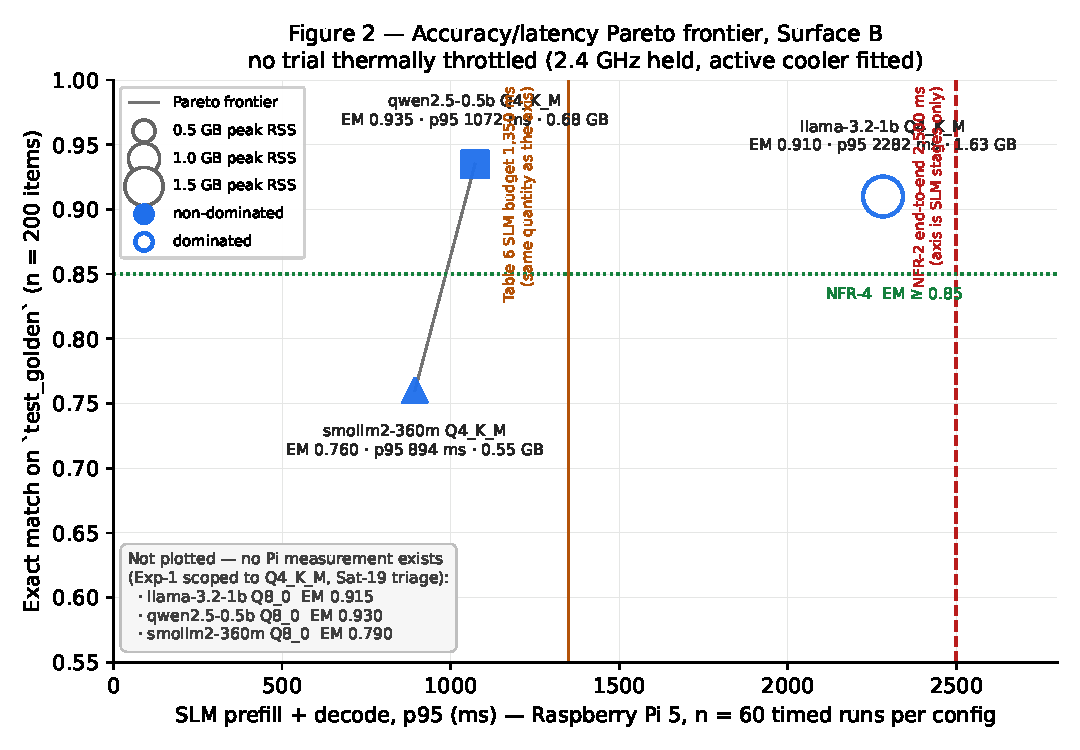
\includegraphics[width=\textwidth]{../results/figure2_pareto.pdf}
  \caption{Figure 2 --- the accuracy--latency Pareto frontier on Surface B, the quantised artefact
  under \texttt{llama.cpp} with the \gls{gbnf} constraint. Vertical axis is exact match on
  \texttt{test\_golden} ($n = 200$ items); horizontal axis is combined \acrshort{slm} prefill and
  decode p95 in milliseconds, measured on the cooled Raspberry~Pi~5 ($n = 60$ timed runs per
  configuration, no trial throttled). Marker area encodes peak resident set size. The solid
  vertical line is Table~6's \acrshort{slm} stage allowance of 1{,}350~ms, which is the same
  quantity as the axis; the dashed line at 2{,}500~ms is NFR-2, an end-to-end budget of which the
  axis measures only a part, so a point left of it has failed to rule itself out rather than passed.
  The horizontal line is NFR-4's exact-match floor of 0.85. Q8\_0 configurations are not plotted:
  Exp-1 was scoped to Q4\_K\_M on hardware, so no Pi latency exists for them. Generated by
  \texttt{eval/plots.py} from \texttt{results/surface\_b.csv} and
  \texttt{results/exp1\_cooled.csv}.}
  \label{fig:pareto}
\end{figure}

\paragraph{NFR-9a is satisfied by every configuration.} Peak resident set size is 0.55~GB, 0.68~GB
and 1.63~GB against a 2.5~GB ceiling. This constraint eliminates nothing.

\paragraph{NFR-2 has not been measured, and cannot be decided here.} NFR-2 bounds end-to-end
latency from end of speech at 2{,}500~ms p95. Exp-1 measures the \acrshort{slm} stages only, and
the remaining stages --- endpointing, \acrshort{stt}, validation and dispatch --- are Exp-2, which
belongs to the \emph{M\'emoire d'Ing\'enieur} and has not run. The constraint can therefore be
applied in one direction only. Because total latency is at least \acrshort{slm} latency on every
trial, the p95 of the total is at least the p95 of the \acrshort{slm} stages, and a configuration
whose \acrshort{slm} p95 already approaches 2{,}500~ms is ruled out without waiting for Exp-2.
Llama-3.2-1B's 2{,}282~ms leaves 218~ms for the rest of a pipeline whose \acrshort{stt} stage alone
is budgeted at 1{,}200~ms: it is eliminated. Qwen2.5-0.5B at 1{,}072~ms and SmolLM2-360M at 894~ms
are not eliminated by this argument, and neither is confirmed by it. This is the sense in which
Figure~\ref{fig:pareto}'s dashed line is drawn but not treated as a verdict.

\paragraph{The rule selects Qwen2.5-0.5B at Q4\_K\_M.} Among the configurations not eliminated,
exact match on the golden split is 0.935 for Qwen2.5-0.5B and 0.760 for SmolLM2-360M, and the rule
ranks on exact match without a tie to break. The selected configuration is also the only one of the
three meeting NFR-4's exact-match floor of 0.85, the 1{,}100~ms decode allowance, the 1{,}350~ms
combined stage allowance, the 20~tok/s throughput floor, NFR-9a and NFR-10 together. SmolLM2-360M
is faster on every timing measure and misses NFR-4 by 9~pp; Llama-3.2-1B is the largest model and
is beaten on accuracy by the model it is eliminated in favour of. Figure~\ref{fig:pareto} shows the
frontier this leaves: Qwen2.5-0.5B and SmolLM2-360M are non-dominated, and Llama-3.2-1B is
dominated on both axes simultaneously.

\paragraph{Three qualifications travel with this selection.} The margin over SmolLM2-360M is
established statistically; the margin over Llama-3.2-1B is not, and the choice between them rests
on the latency constraint rather than on the accuracy difference, which
Section~\ref{sec:statistics} declines to call real. The selection is made against reference-text
accuracy, and Section~\ref{sec:exp0} bounds how much of that accuracy the acoustic front end will
consume. And the selected configuration, like every other one measured, misses NFR-9 and NFR-18:
it is selected as the best available on the criteria the rule names, not as a configuration that
satisfies every requirement placed on the system. The discussion chapter takes up what that
costs and what it would take to fix. % \ref{chap:discussion} once ch5 exists
      % Results: Exp-0; Exp-1; quantisation delta;
%                                 % grammar ablation; statistics; selection rule
% \chapter{Discussion and limitations}
\label{chap:discussion}

% Scaffold from prd.md 3.1: the accuracy--efficiency trade-off characterised as a Pareto
% frontier; failure-mode analysis; threats to internal and external validity.
% Register: hedged and exploratory. Chapter 4 reported; this chapter interprets. The verdict
% on RQ1 belongs to Chapter 6 and is not pre-empted here.

\TODO{Chapter lead-in, written last: what this chapter interprets, and what it leaves to
Chapter~\ref{chap:conclusion}.}

\section{The accuracy--efficiency trade-off}
\label{sec:tradeoff}

RQ1 was posed as a trade-off: across the 0.36--1.2~B range, how much task accuracy does a smaller
model give up in exchange for latency and memory? Figure~\ref{fig:pareto} gives the measured
answer for this task and this board. The answer turns out to have less of the shape of a
trade-off than the question anticipated.

\paragraph{A frontier of two points.} Only three configurations have both an accuracy and a
latency coordinate, and one of them, Llama-3.2-1B at Q4\_K\_M, is dominated. The frontier is
therefore the pair \{SmolLM2-360M, Qwen2.5-0.5B\}, and a pair defines a direction, not a curve.
Moving along it from Qwen2.5-0.5B to SmolLM2-360M saves 178~ms of combined \acrshort{slm} p95
(1{,}072~ms to 894~ms) and 0.13~GB of peak resident memory, and costs 17.5~pp of exact match on the
golden split. That accuracy cost is the one difference in this study that the paired tests
establish decisively (Section~\ref{sec:statistics}). Moving the other way, from Qwen2.5-0.5B to
Llama-3.2-1B, adds 1{,}210~ms and 0.95~GB, and the accuracy difference it buys is not
distinguishable from zero on this evidence. Read together, the two directions suggest that for
this schema the useful part of the range ends at or below half a billion parameters. Below that
point accuracy falls steeply. Above it, parameters appear to purchase latency and memory and
little else. With three points on the latency axis this is a reading of the figure's shape, not a
measured property of the size range, and it should be held at that strength.

\paragraph{The knee belongs to a model, not to a size.} It would be tempting to restate the
previous paragraph as ``0.5~B parameters suffice''. The iso-parameter control of
Section~\ref{sec:iso-parameter} argues against that restatement. H2O-Danube3-500M, within 4.0\% of
Qwen2.5-0.5B's parameter count, scores 6.5~pp lower on the golden split at FP16. It has no latency
coordinate, because it has no quantised artefact, so it cannot be placed on
Figure~\ref{fig:pareto}. What it does show is that at a fixed size the vertical position of a point
can move by more than a third of the distance separating the two frontier models. The frontier's knee
therefore sits at Qwen2.5-0.5B specifically, and whether another family at the same size would sit
on it, above it or below it is not something these data decide. A practitioner reusing this result
should read it as a statement about a model that was measured, not about a parameter class.

\paragraph{The selection rule faced a feasibility cut, not a trade.} The rule in
Section~\ref{sec:selection} ranks the configurations by exact match after the constraints have
been applied. In principle a Pareto frontier forces a choice of operating point along it. Here the
choice was never exercised. The only configuration faster than the selected one scores 0.760,
which is under NFR-4's floor of 0.85 by 9~pp, so NFR-4 rules it out even though the selection rule
itself does not rank on NFR-4. Of the three measured configurations, then, one is dominated, one
is too inaccurate to deploy, and one remains. RQ1's trade-off exists on the figure, but it does
not reach the deployment decision. The obvious caution applies: this is a consequence of which
three models were measured. A model faster than SmolLM2-360M that cleared the 0.85 floor would
reopen the choice, and nothing measured here rules such a model out.

\paragraph{How much of the horizontal axis belongs to the enclosure.} The latency coordinates in
Figure~\ref{fig:pareto} are measured on a cooled board, and Table~\ref{tab:thermal-headroom} shows
how far they move without the cooler. Uncooled, the selected configuration's combined
\acrshort{slm} p95 is 1{,}771.5~ms. That is over the 1{,}350~ms stage allowance of
Table~\ref{tab:latency-budget}, and so is SmolLM2-360M's 1{,}610.2~ms. On the uncooled run no
configuration meets the stage allowance, and the feasible set that the selection draws from is
empty. The selected configuration is therefore feasible only because the board is cooled, and its
margin on the cooled board is modest. The combined stage is 278~ms inside its allowance, but
decode alone is 1{,}033~ms against 1{,}100~ms, a margin of 67~ms or 6\%. A frontier drawn on
this class of hardware is conditional on its thermal state. The figure is best read as the
frontier of a cooled Raspberry~Pi~5, and not as a frontier of the three models in the abstract.

\paragraph{What would move the frontier.} Two gaps in the figure are known, and each limits what
the frontier can be taken to mean. The first is quantisation. The Q8\_0 artefacts have no
latency coordinate, and the paired tests found no accuracy difference between quantisations
within any model. A Q8\_0 point could join the frontier only by matching or beating its
Q4\_K\_M counterpart on latency. That was not measured, so the frontier is strictly a Q4\_K\_M
frontier. The second is the horizontal axis itself, which covers the \acrshort{slm} stages only.
The remaining stages of the pipeline run the same software whichever model is loaded, so adding
them may shift all three points to the right by comparable amounts. If so, the ordering along the
frontier would survive and the absolute margins would not. That is a plausible expectation rather
than a measured one. The stages share one board's processor, and a larger model could slow them
through contention, so whether the selected configuration remains feasible against the end-to-end
budget is a question this document leaves open.

\section{Failure-mode analysis}
\label{sec:failure-modes}

% Inherits results/limitation_abstention.md (NFR-9 / NFR-18) -- cited, not re-derived.
% The grammar guarantees structure, not abstention. The grammar-ablation reading cut from
% Ch4 (fine-tune left the grammar 0.17 pp; same training removed abstention) is a HYPOTHESIS.
% Yaw sign flip as the largest in-domain family, invisible to every validation layer.
\TODO{Section 5.2.}

\section{Threats to validity}
\label{sec:threats}

\subsection{Internal validity}
\label{sec:threats-internal}

% The three Danube deviations (system-role fold, separate session, Surface A only after the
% Gate 3 tokeniser failure). The zero-shot baseline: no causal claim, predictions not
% retained. SmolLM2's cooled gain (1.69x) exceeding the 1.6x clock ratio, term unidentified.
% Fixed three-epoch budget; n = 200 golden items; single recording session.
\TODO{Section 5.3.1.}

\subsection{External validity}
\label{sec:threats-external}

% Exp-3 referenced EXACTLY ONCE, here, as external validity for the deployed model, naming
% the Memoire d'Ingenieur (prd.md Table 3). Single speaker; one board; small schema.
\TODO{Section 5.3.2.}
   % Discussion and limitations: Pareto frontier;
%                                 % failure modes; threats to validity
% \chapter{Conclusion and future work}
\label{chap:conclusion}

This chapter closes the comparison. Section~\ref{sec:rq1-answer} answers RQ1 against the results
of Chapter~\ref{chap:results} and states where the selected configuration stands against the
requirements it was selected under. Section~\ref{sec:established} sets out what the comparison
establishes for each contribution of Chapter~\ref{chap:introduction}, at the strength the results
support. Section~\ref{sec:next-steps} names the steps that follow from them, in order of priority.

% -----------------------------------------------------------------------------
% Register: unhedged. Every number already appears in Chapter 4 (or STATE.md) with
% the same value and the same qualifier; unhedged means no hedging words, not
% stronger claims. No new caveat belongs here: a limitation found while drafting
% goes to Chapter 5.
% -----------------------------------------------------------------------------

\section{Answer to the research question}
\label{sec:rq1-answer}

Across fine-tuned \glspl{slm} of 0.36--1.2~B parameters quantised for a Raspberry~Pi~5,
the accuracy--efficiency trade-off reduces to two non-dominated configurations, SmolLM2-360M and
Qwen2.5-0.5B, and the selection rule deploys Qwen2.5-0.5B at Q4\_K\_M, at 0.935 \gls{em} on the
golden split. Between the two, the trade-off has a measured price. On the cooled board, SmolLM2-360M
completes the \gls{slm} stages at a p95 of 894~ms against Qwen2.5-0.5B's 1{,}072~ms, and it scores
0.760, 17.5~pp lower, a gap significant at the corrected $\alpha$ (Section~\ref{sec:statistics}).
On the split the rule ranks on, the largest model buys no established accuracy. Llama-3.2-1B, at
1.24~B parameters, scores 0.910 there, a difference from Qwen2.5-0.5B that the test does not
establish, and takes 2{,}282~ms, so it is dominated on latency.

Qwen2.5-0.5B is selected on accuracy, against constraints re-baselined under the rule's failure
clause (Section~\ref{sec:selection}). It misses the 2{,}500~ms end-to-end budget as specified by
622~ms (25\%), and the budget is re-baselined to its measured p95 of 3{,}122~ms. The memory
ceiling is confirmed for the language-model process only, at 0.68~GiB against 2.5~GiB. The
selection does not depend on SmolLM2-360M's end-to-end latency, which was not measured: admitting
SmolLM2-360M leaves it unchanged, because Qwen2.5-0.5B's margin over it is significant. Its margin
over Llama-3.2-1B is not, and the choice between those two rests on latency. Like every
configuration measured, Qwen2.5-0.5B misses both abstention requirements. Across the six
configurations, the safe-failure rate is 0.0000--0.1579 against a budget of $\geq$~0.70, and the
false-command rate on out-of-domain input is 0.1867--0.3933 against $\leq$~0.05: when wrong or out
of domain, the parser emits a well-formed command rather than \texttt{unknown}. Qwen2.5-0.5B at
Q4\_K\_M is the best configuration measured on the criteria the selection rule names; it does not
meet every requirement placed on the system.

\section{What the comparison establishes}
\label{sec:established}

The grammar makes structural validity a property of the decoder (Contribution~C1). Schema validity
is 1.000 on all eighteen rows of the multi-model benchmark, and it moves only when the grammar is
removed: over 3{,}540 decodes without it, exactly one output is malformed and \gls{em} falls by
0.17~pp (Section~\ref{sec:grammar-ablation}). Two results follow, and they are distinct. On these
test splits, the fine-tuned models depart from the format once in 3{,}540 decodes when nothing
prevents them, so the grammar's measurable contribution to validity is that one decode. The
property the grammar provides is of another kind: no token sequence violating the schema is
reachable under the constraint, for any input, and no rate on a finite test set measures it. The
grammar also carries no measured accuracy cost on this schema, the 0.17~pp difference falling in
its favour.

None of the accuracy the comparison reports is available from the pretrained models as prompted
(Contribution~C2). Prompted zero-shot at fp16, without fine-tuning and without the grammar, the
four models match none of the 590 items on any split (Section~\ref{sec:iso-parameter}); fine-tuned
on the label-first corpus and decoded under the grammar, the selected model reaches 0.935 on the
golden split. The zero-shot rows remove the fine-tune and the grammar together, so they fix the
baseline the fine-tune is measured from and do not attribute the gain to either intervention.

The harness measures the accuracy cost of the deployment pipeline on this task, and on 200 items it
does not separate that cost from zero (Contribution~C3). From each fp16 model on the reference
surface to its quantised artefacts on the deployed surface, \gls{em} on the golden split moves by
$-$1.5 to $+$1.5~pp, no difference exceeds three items net, and none is significant in the
exploratory family, whose smallest $p$ is 0.25 (Section~\ref{sec:quantisation-delta}). Precision,
runtime and grammar change together between the two surfaces, so the figure is the cost of the
pipeline as a whole, not of quantisation. The latency results hold for a cooled board: without
active cooling, every trial throttled, and fitting the cooler reduced decode p95 by 25.1\% to
41.3\% (Section~\ref{sec:benchmark}).

At matched size, model family moves \gls{em} by 6.5~pp: at about 0.5~B parameters, Qwen2.5-0.5B
scores 0.935 against H2O-Danube3-500M's 0.870, on 15 against 2 discordant items (exact
$p = 0.0023$, an exploratory test), under the identical three-epoch budget at which no model is
shown to have converged (Section~\ref{sec:iso-parameter}). Among the three deployed models, size
and family vary together, so the comparison measures a family difference at fixed size and does
not express it as a share of a size effect.

\section{Prioritised next steps}
\label{sec:next-steps}

Three steps follow from these results, ordered by the requirement each addresses. None of them is
implemented or measured in this document.

\begin{enumerate}
  \item \textbf{A confidence gate.} The two abstention requirements are the ones the selected
  configuration misses by the widest margin (Section~\ref{sec:benchmark}), and a gate addresses
  them without retraining. It reads the decoder's token-level log-probabilities over the emitted
  command and routes any command below a threshold to \texttt{unknown} rather than to dispatch,
  which targets the in-domain errors of Section~\ref{sec:failure-modes}: the parser dispatches them
  as executable commands instead of declining. The threshold is placed on a held-out calibration
  set, not on the golden split, and it trades safe-failure rate against \gls{em} along a curve that
  is the first measurement to make.
  \item \textbf{Training pairs for unreadable commands.} The corpus teaches \texttt{unknown}
  through 81 pairs, none of them a supported command made unreadable by recognition error
  (Section~\ref{sec:dataset}). Pairs of that kind change what the model treats as an available
  answer on in-domain input, where the gate changes only what is dispatched, so the two steps are
  complementary. This one requires retraining and a second run of the multi-model benchmark.
  \item \textbf{An end-to-end measurement of SmolLM2-360M.} SmolLM2-360M is the one
  non-dominated configuration shown neither to satisfy the end-to-end budget nor to miss it, and
  no configuration's full-stack memory was measured. Measuring both for SmolLM2-360M completes the
  frontier of Section~\ref{sec:rq1-answer} at its fast end. The selection does not depend on the
  outcome.
\end{enumerate}
   % Conclusion and future work: RQ1 answered

% -- Bibliography -------------------------------------------------------------
\newpage
\printbibliography
\addcontentsline{toc}{chapter}{Bibliography}

\end{document}
